% One-sided layout for bachelor thesis
\documentclass[headsepline,footsepline,footinclude=false,oneside,fontsize=11pt,paper=a4,listof=totoc,bibliography=totoc,DIV=12]{scrbook}

\usepackage{algorithm}
\usepackage{algpseudocode}
\RequirePackage[l2tabu,orthodox]{nag}

\PassOptionsToPackage{table,svgnames,dvipsnames}{xcolor}

\usepackage[utf8]{inputenc}
\usepackage[T1]{fontenc}
\usepackage[sc]{mathpazo}
\usepackage[ngerman,english]{babel} % english is the same as american or USenglish
\usepackage[autostyle]{csquotes}
\usepackage[%
  backend=biber,
  url=true,
  style=numeric, % alphabetic, numeric
  sorting=none, % default == nty, https://tex.stackexchange.com/questions/51434/biblatex-citation-order
  maxnames=4,
  minnames=3,
  maxbibnames=99,
  giveninits,
  uniquename=init]{biblatex} % TODO: adapt citation style
\usepackage{graphicx}
\usepackage{scrhack} % necessary for listings package
\usepackage{listings}
\usepackage{lstautogobble}
\usepackage{tikz}
\usepackage{pgfplots}
\usepackage{pgfplotstable}
\usepackage{booktabs} % for better looking table creations, but bad with vertical lines by design (package creator despises vertical lines)
\usepackage[final]{microtype}
\usepackage{caption}
\usepackage[hidelinks]{hyperref} % hidelinks removes colored boxes around references and links
\usepackage{ifthen} % for comparison of the current language and changing of the thesis layout
\usepackage{pdftexcmds} % string compare to work with all engines
\usepackage{paralist} % for condensed enumerations or lists
\usepackage{subfig} % for having figures side by side
\usepackage{siunitx} % for physical accurate units and other numerical presentations
\usepackage{multirow} % makes it possible to have bigger cells over multiple rows in a table
\usepackage{array} % different options for table cell orientation
\usepackage{makecell} % allows nice manual configuration of cells with linebreaks in \thead and \makecell with alignments
\usepackage{pdfpages} % for including multiple pages of pdfs
\usepackage{adjustbox} % can center content wider than the \textwidth
\usepackage{tablefootnote} % for footnotes in tables as \tablefootnote
\usepackage{threeparttable} % another way to add footnotes as \tablenotes with \item [x] <your footnote> after setting \tnote{x} 


% https://tex.stackexchange.com/questions/42619/x-mark-to-match-checkmark
\usepackage{amssymb}% http://ctan.org/pkg/amssymb
\usepackage{pifont}% http://ctan.org/pkg/pifont
\newcommand{\cmark}{\ding{51}}%
\newcommand{\xmark}{\ding{55}}%


\usepackage[acronym,xindy,toc]{glossaries} % TODO: include "acronym" if glossary and acronym should be separated
\makeglossaries
\loadglsentries{pages/glossary.tex} % important update for glossaries, before document


\bibliography{bibliography}

\setkomafont{disposition}{\normalfont\bfseries} % use serif font for headings
\linespread{1.05} % adjust line spread for mathpazo font

% Add table of contents to PDF bookmarks
\BeforeTOCHead[toc]{{\cleardoublepage\pdfbookmark[0]{\contentsname}{toc}}}

% Define TUM corporate design colors
% Taken from http://portal.mytum.de/corporatedesign/index_print/vorlagen/index_farben
\definecolor{TUMBlue}{HTML}{0065BD}
\definecolor{TUMSecondaryBlue}{HTML}{005293}
\definecolor{TUMSecondaryBlue2}{HTML}{003359}
\definecolor{TUMBlack}{HTML}{000000}
\definecolor{TUMWhite}{HTML}{FFFFFF}
\definecolor{TUMDarkGray}{HTML}{333333}
\definecolor{TUMGray}{HTML}{808080}
\definecolor{TUMLightGray}{HTML}{CCCCC6}
\definecolor{TUMAccentGray}{HTML}{DAD7CB}
\definecolor{TUMAccentOrange}{HTML}{E37222}
\definecolor{TUMAccentGreen}{HTML}{A2AD00}
\definecolor{TUMAccentLightBlue}{HTML}{98C6EA}
\definecolor{TUMAccentBlue}{HTML}{64A0C8}

% Settings for pgfplots
\pgfplotsset{compat=newest}
\pgfplotsset{
  % For available color names, see http://www.latextemplates.com/svgnames-colors
  cycle list={TUMBlue\\TUMAccentOrange\\TUMAccentGreen\\TUMSecondaryBlue2\\TUMDarkGray\\},
}

% Settings for lstlistings

% Use this for basic highlighting
\lstset{%
  basicstyle=\ttfamily,
  columns=fullflexible,
  autogobble,
  keywordstyle=\bfseries\color{TUMBlue},
  stringstyle=\color{TUMAccentGreen}
}

% use this for C# highlighting
% %\setmonofont{Consolas} %to be used with XeLaTeX or LuaLaTeX
% \definecolor{bluekeywords}{rgb}{0,0,1}
% \definecolor{greencomments}{rgb}{0,0.5,0}
% \definecolor{redstrings}{rgb}{0.64,0.08,0.08}
% \definecolor{xmlcomments}{rgb}{0.5,0.5,0.5}
% \definecolor{types}{rgb}{0.17,0.57,0.68}

% \lstset{language=[Sharp]C,
% captionpos=b,
% %numbers=left, % numbering
% %numberstyle=\tiny, % small row numbers
% frame=lines, % above and underneath of listings is a line
% showspaces=false,
% showtabs=false,
% breaklines=true,
% showstringspaces=false,
% breakatwhitespace=true,
% escapeinside={(*@}{@*)},
% commentstyle=\color{greencomments},
% morekeywords={partial, var, value, get, set},
% keywordstyle=\color{bluekeywords},
% stringstyle=\color{redstrings},
% basicstyle=\ttfamily\small,
% }

% Settings for search order of pictures
\graphicspath{
    {logos/}
    {figures/}
}

% Set up hyphenation rules for the language package when mistakes happen
\babelhyphenation[english]{
an-oth-er
ex-am-ple
}

% Decide between
%\newcommand{\todo}[1]{\textbf{\textsc{\textcolor{TUMAccentOrange}{(TODO: #1)}}}} % for one paragraph, otherwise error!
%\newcommand{\done}[1]{\textit{\textsc{\textcolor{TUMAccentBlue}{(Done: #1)}}}} % for one paragraph, otherwise error!
% and
\newcommand{\todo}[1]{{\bfseries{\scshape{\color{TUMAccentOrange}[(TODO: #1)]}}}} % for multiple paragraphs
\newcommand{\done}[1]{{\itshape{\scshape{\color{TUMAccentBlue}[(Done: #1)]}}}} % for multiple paragraphs
% for error handling of intended behavior in your latex documents.

\newcommand{\tabitem}{~~\llap{\textbullet}~~}

\newcolumntype{P}[1]{>{\centering\arraybackslash}p{#1}} % for horizontal alignment with limited column width
\newcolumntype{M}[1]{>{\centering\arraybackslash}m{#1}} % for horizontal and vertical alignment with limited column width
\newcolumntype{L}[1]{>{\raggedright\arraybackslash}m{#1}} % for vertical alignment left with limited column width
\newcolumntype{R}[1]{>{\raggedleft\arraybackslash}m{#1}} % for vertical alignment right with limited column width 

% Thesis information
\newcommand*{\getUniversity}{Technische Universität München}
\newcommand*{\getFaculty}{Department of Informatics}
\newcommand*{\getTitle}{Topic: Enhancing Intraoperative Registration with Neural Radiance Fields: An Exploration of Loss Functions Effects}
\newcommand*{\getTitleGer}{Verbesserung der intraoperativen Registrierung mit Neural Radiance Fields: Eine Untersuchung der Auswirkungen von Verlustfunktionen}
\newcommand*{\getAuthor}{Davyd Podolskyi}
\newcommand*{\getDoctype}{Bachelor's Thesis in Informatics}
\newcommand*{\getSupervisor}{Prof. Dr. Nassir Navab}
\newcommand*{\getAdvisorTUM}{Mohammad Farid Azampour, M.Sc.}
\newcommand*{\getAdvisorHarvard}{Nazim Haouchine, PhD.}
\newcommand*{\getSubmissionDate}{18.03.2025}
\newcommand*{\getSubmissionLocation}{Munich}

% Add bibliography file
\addbibresource{bibliography.bib}

\begin{document}

% English as main language
\selectlanguage{english}

% Set page numbering to avoid "destination with the same identifier has been already used" warning for cover page.
\pagenumbering{alph}
\begin{titlepage}
  % HACK for two-sided documents: ignore binding correction for cover page.
  % Adapted from Markus Kohm's KOMA-Script titlepage=firstiscover handling.
  % See http://mirrors.ctan.org/macros/latex/contrib/koma-script/scrkernel-title.dtx,
  % \maketitle macro.
  \oddsidemargin=\evensidemargin\relax
  \textwidth=\dimexpr\paperwidth-2\evensidemargin-2in\relax
  \hsize=\textwidth\relax

  \centering

  \IfFileExists{logos/tum.pdf}{%
    
\includegraphics[height=20mm]{logos/tum.pdf}
  }{%
    \vspace*{20mm}
  }

  \vspace{5mm}
  {\huge\MakeUppercase{\getFaculty{}}}\\

  \vspace{5mm}
  {\large\MakeUppercase{\getUniversity{}}}\\

  \vspace{20mm}
  {\Large \getDoctype{}}

  \vspace{15mm}
  \makeatletter
  \ifthenelse{\pdf@strcmp{\languagename}{english}=0}
  {\huge\bfseries \getTitle{}}
  {\huge\bfseries \getTitleGer{}}
  \makeatother

  \vspace{15mm}
  {\LARGE \getAuthor{}}

\end{titlepage}


\frontmatter{}

\begin{titlepage}
  \centering

  \IfFileExists{logos/tum.pdf}{%
    
\includegraphics[height=20mm]{logos/tum.pdf}
  }{%
    \vspace*{20mm}
  }

  \vspace{5mm}
  {\huge\MakeUppercase{\getFaculty{}}}\\

  \vspace{5mm}
  {\large\MakeUppercase{\getUniversity{}}}\\

  \vspace{20mm}
  {\Large \getDoctype{}}

  \makeatletter
  \vspace{15mm}
  \ifthenelse{\pdf@strcmp{\languagename}{english}=0}
  {
  {\huge\bfseries \getTitle{}}

  \vspace{10mm}
  {\huge\bfseries \foreignlanguage{ngerman}{\getTitleGer{}}}
  }
  {
  {\huge\bfseries \getTitleGer{}}

  \vspace{10mm}
  {\huge\bfseries \foreignlanguage{english}{\getTitle{}}}
  }
  \makeatother

  \vspace{15mm}
  \begin{tabular}{l l}
    Author:          & \getAuthor{} \\
    Supervisor, TUM:      & \getSupervisor{} \\
    Advisor, TUM: & \getAdvisorTUM{} \\
    Advisor, Harvard Medical School: & \getAdvisorHarvard{} \\
    Submission Date: & \getSubmissionDate{} \\
  \end{tabular}

  
\end{titlepage}

\cleardoublepage{}

\thispagestyle{empty}
\vspace*{0.6\textheight}
\noindent
\makeatletter
\ifthenelse{\pdf@strcmp{\languagename}{english}=0}
{I confirm that this bachelor’s thesis is my own work and I have documented all sources and material used. \\ \\
Ich versichere, dass ich diese Bachelor’s Thesis selbständig verfasst und nur die angegebenen Quellen und Hilfsmittel verwendet habe.}
\makeatother

\vspace{15mm}
\noindent
\getSubmissionLocation{}, \getSubmissionDate{} \hspace{50mm} \getAuthor{}

\cleardoublepage{}

\makeatletter
\ifthenelse{\pdf@strcmp{\languagename}{english}=0}
{\addcontentsline{toc}{chapter}{Acknowledgments}}
{\addcontentsline{toc}{chapter}{Danksagungen}}
\makeatother
\thispagestyle{empty}

\vspace*{20mm}

\begin{center}
\makeatletter
\ifthenelse{\pdf@strcmp{\languagename}{english}=0}
{\usekomafont{section} Acknowledgments}
{\usekomafont{section} Danksagungen}
\makeatother
\end{center}

\vspace{10mm}

\chapter*{Acknowledgements}

I would like to express my sincere gratitude to everyone who supported me throughout the journey of completing this thesis.

First and foremost, I would like to thank my supervisor, Prof. Dr. Nassir Navab, for providing me with the opportunity to work on this exciting research topic at the Computer Aided Medical Procedures (CAMP) chair. His guidance, expertise, and vision in the field of medical image computing have been invaluable to this work.

I am deeply grateful to my advisor, Maximilian Fehrentz, for his continuous support, patience, and mentorship. His pioneering work on cross-modal neural rendering for intraoperative registration laid the foundation for this thesis, and his detailed feedback and insightful discussions have significantly shaped and improved my research.

I would also like to extend my appreciation to the entire CAMP team for creating a collaborative and stimulating research environment. The weekly seminars, discussions, and exchange of ideas have been incredibly helpful in refining my approach and broadening my perspective.

Special thanks to the clinical partners at the University Hospital for providing access to the clinical datasets used in this research and for sharing their valuable medical expertise. Their insights into the practical challenges of neurosurgical navigation have been essential in guiding this work toward clinical relevance.

I am thankful to my fellow students and friends who have contributed to this work through technical discussions, proofreading, and moral support. Their camaraderie made the challenging moments more bearable and the successes more enjoyable.

Finally, I would like to express my heartfelt gratitude to my family for their unwavering support, encouragement, and understanding throughout my academic journey. Their belief in me has been a constant source of motivation.

This thesis was partially supported by the Technical University of Munich and the CAMP chair, which provided the computational resources and academic environment necessary for this research.

\vspace{1cm}
\begin{flushright}
David\\
Munich, September 2023
\end{flushright}

\cleardoublepage{}

\chapter{\abstractname}

This study advances intraoperative brain registration using Neural Radiance Fields (NeRFs) as learned functional representations of brain surfaces. Unlike traditional mesh-based approaches, NeRFs provide a differentiable, implicit function of the brain's geometry and appearance. We leverage this property to optimize camera positions through backpropagation, enabling precise alignment of preoperative and intraoperative brain images. Our research explores various loss functions (Mutual Information, Normalized Cross-Correlation, weighted/masked L2) and analyzes the impact of hypernetwork-generated styles on registration accuracy. By enhancing NeRF-based brain registration, this work aims to improve the precision of image-guided neurosurgery.



\makeatletter
\ifthenelse{\pdf@strcmp{\languagename}{english}=0}
{\renewcommand{\abstractname}{Kurzfassung}}
{\renewcommand{\abstractname}{Abstract}}
\makeatother

\chapter{\abstractname}

\begin{otherlanguage}{ngerman}
Diese Studie verbessert die intraoperative Hirnregistrierung durch den Einsatz von Neural Radiance Fields (NeRFs) als erlernte funktionale Darstellungen von Hirnoberflächen. Im Gegensatz zu traditionellen netzbasierten Ansätzen bieten NeRFs eine differenzierbare, implizite Funktion der Geometrie und des Erscheinungsbilds des Gehirns. Wir nutzen diese Eigenschaft, um Kamerapositionen durch Backpropagation zu optimieren und ermöglichen so eine präzise Ausrichtung von präoperativen und intraoperativen Hirnbildern. Unsere Forschung untersucht verschiedene Verlustfunktionen (Mutual Information, Normalized Cross-Correlation, gewichteter/maskierter L2-Verlust) und analysiert den Einfluss von durch Hypernetzwerke generierte Stile auf die Registrierungsgenauigkeit. Durch die Verbesserung der NeRF-basierten Hirnregistrierung zielt diese Arbeit darauf ab, die Präzision der bildgeführten Neurochirurgie zu verbessern.
\end{otherlanguage}


% Undo the name switch
\makeatletter
\ifthenelse{\pdf@strcmp{\languagename}{english}=0}
{\renewcommand{\abstractname}{Abstract}}
{\renewcommand{\abstractname}{Kurzfassung}}
\makeatother
\microtypesetup{protrusion=false}
\tableofcontents{}
\microtypesetup{protrusion=true}

\mainmatter{}

% !TeX root = ../main.tex
% Add the above to each chapter to make compiling the PDF easier in some editors.

\chapter{Introduction}\label{chapter:introduction}

Neurosurgery is a high-precision medical field where accuracy is paramount to patient outcomes. During brain tumor resection procedures, surgeons rely on image-guided navigation systems to assist with spatial orientation and to locate critical structures within the brain \parencite{navab2015surgical}. These systems typically align preoperative Magnetic Resonance Imaging (MRI) data with the patient's physical anatomy through a process called registration. Traditional registration methods often employ point-based or surface-based techniques, which can be time-consuming, require specialized equipment, and are susceptible to inaccuracies due to brain shift—the deformation of brain tissue that occurs once the skull is opened.

The field of computer vision has recently seen remarkable advancements in neural scene representation techniques, particularly with the introduction of Neural Radiance Fields (NeRFs) \parencite{mildenhall2020nerf}. NeRFs represent scenes as continuous functions that map 3D coordinates and viewing directions to color and density values, enabling high-quality novel view synthesis. These implicit neural representations have revolutionized how we model and render 3D environments, offering differentiable, continuous scene representations that can be optimized through gradient-based methods.

This thesis builds upon recent work that leverages NeRFs for pose estimation \parencite{yen2020inerf} and, more specifically, for intraoperative registration \parencite{fehrentz2024intraoperative}. We propose to enhance NeRF-based intraoperative registration through two main contributions: (1) a comprehensive exploration of alternative loss functions beyond the standard L2 loss, and (2) an investigation into the effects of style transfer on registration accuracy.

\section{Motivation}

Current intraoperative registration techniques face several challenges:

\begin{enumerate}
    \item \textbf{Brain shift}: The brain's position and shape change during surgery due to cerebrospinal fluid drainage, gravity, and surgical manipulations.
    \item \textbf{Cross-modal alignment}: Matching preoperative MRI data with intraoperative camera images requires bridging different imaging modalities.
    \item \textbf{Speed and accuracy}: Registration must be both precise and fast enough to be clinically viable during surgery.
    \item \textbf{Surgical workflow integration}: Registration methods should integrate seamlessly into existing surgical workflows without requiring additional equipment or extensive time.
\end{enumerate}

The approach presented by \textcite{fehrentz2024intraoperative} addresses these challenges by using neural rendering for registration. However, their work primarily focuses on a hypernetwork-based approach for appearance adaptation and employs a standard L2 loss for optimization. This thesis extends their work by exploring whether alternative loss functions might yield better registration results and by analyzing how different style transfer techniques affect the registration process.

\section{Research Questions}

This thesis addresses the following key research questions:

\begin{enumerate}
    \item How do different loss functions (Mutual Information, Normalized Cross-Correlation, and weighted/masked L2) compare to the standard L2 loss in NeRF-based intraoperative registration?
    \item What impact do various hypernetwork-generated styles have on registration accuracy when using NeRF-based methods?
    \item Can the combination of specific loss functions and style transfer techniques improve registration robustness against variations in lighting, perspective, and tissue appearance?
\end{enumerate}

\section{Contributions}

The main contributions of this thesis are:

\begin{enumerate}
    \item A systematic evaluation of multiple loss functions for NeRF-based intraoperative registration.
    \item An analysis of hypernetwork-based style transfer effects on registration accuracy.
    \item An implementation built on top of nerfstudio to make the approach NeRF-implementation agnostic.
    \item Experimental results comparing different combinations of loss functions and style transfer techniques.
\end{enumerate}

\section{Thesis Structure}

The remainder of this thesis is organized as follows:

\begin{itemize}
    \item \textbf{Chapter~\ref{chapter:background}}: Provides the necessary background on neural radiance fields, pose estimation, and intraoperative registration.
    \item \textbf{Chapter~\ref{chapter:methodology}}: Explains the methodology and overall approach for NeRF-based registration.
    \item \textbf{Chapter~\ref{chapter:loss_functions}}: Details the loss functions implemented and evaluated in this work.
    \item \textbf{Chapter~\ref{chapter:style_transfer}}: Explores the style transfer techniques and their integration with the registration process.
    \item \textbf{Chapter~\ref{chapter:experiments}}: Describes the experimental setup, datasets, and evaluation metrics.
    \item \textbf{Chapter~\ref{chapter:results}}: Presents the results of our experiments and analyses.
    \item \textbf{Chapter~\ref{chapter:discussion}}: Discusses the implications of our findings and their relevance to the field.
    \item \textbf{Chapter~\ref{chapter:conclusion}}: Summarizes the thesis and suggests directions for future research.
\end{itemize}

\section{Section}
Citation test (with Biber)~\parencite{latex}.

\subsection{Subsection}

See~\autoref{tab:sample}, \autoref{fig:sample-drawing}, \autoref{fig:sample-plot}, \autoref{fig:sample-listing}, \autoref{fig:tum}, \autoref{fig:tumslide}.

\begin{table}[htpb]
  \caption[Example table]{An example for a simple table.}\label{tab:sample}
  \centering
  \begin{tabular}{l l l l}
    \toprule
      A & B & C & D \\
    \midrule
      1 & 2 & 1 & 2 \\
      2 & 3 & 2 & 3 \\
    \bottomrule
  \end{tabular}
\end{table}

\begin{figure}[htpb]
  \centering
  % This should probably go into a file in figures/
  \begin{tikzpicture}[node distance=3cm]
    \node (R0) {$R_1$};
    \node (R1) [right of=R0] {$R_2$};
    \node (R2) [below of=R1] {$R_4$};
    \node (R3) [below of=R0] {$R_3$};
    \node (R4) [right of=R1] {$R_5$};

    \path[every node]
      (R0) edge (R1)
      (R0) edge (R3)
      (R3) edge (R2)
      (R2) edge (R1)
      (R1) edge (R4);
  \end{tikzpicture}
  \caption[Example drawing]{An example for a simple drawing.}\label{fig:sample-drawing}
\end{figure}

\begin{figure}[htpb]
  \centering

  \pgfplotstableset{col sep=&, row sep=\\}
  % This should probably go into a file in data/
  \pgfplotstableread{
    a & b    \\
    1 & 1000 \\
    2 & 1500 \\
    3 & 1600 \\
  }\exampleA
  \pgfplotstableread{
    a & b    \\
    1 & 1200 \\
    2 & 800 \\
    3 & 1400 \\
  }\exampleB
  % This should probably go into a file in figures/
  \begin{tikzpicture}
    \begin{axis}[
        ymin=0,
        legend style={legend pos=south east},
        grid,
        thick,
        ylabel=Y,
        xlabel=X
      ]
      \addplot table[x=a, y=b]{\exampleA};
      \addlegendentry{Example A};
      \addplot table[x=a, y=b]{\exampleB};
      \addlegendentry{Example B};
    \end{axis}
  \end{tikzpicture}
  \caption[Example plot]{An example for a simple plot.}\label{fig:sample-plot}
\end{figure}

\begin{figure}[htpb]
  \centering
  \begin{tabular}{c}
  \begin{lstlisting}[language=SQL]
    SELECT * FROM tbl WHERE tbl.str = "str"
  \end{lstlisting}
  \end{tabular}
  \caption[Example listing]{An example for a source code listing.}\label{fig:sample-listing}
\end{figure}

\begin{figure}[htpb]
  \centering
  
\includegraphics[width=0.8\textwidth]{tum}
  \caption[Something else can be written here for listing this, otherwise the caption will be written!]{Includegraphics searches for the filename without extension first in logos, then in figures.} \label{fig:tum}
\end{figure}

\begin{figure}[htpb]
  \centering
  
\includegraphics[width=0.8\textwidth]{figures/tum}
  \caption{For pictures with the same name, the direct folder needs to be chosen.} \label{fig:tumslide}
\end{figure}

\begin{figure}[!tbp]
  \centering
  \subfloat[TUM Logo][The logo.]{
\includegraphics[height=0.2\textheight]{tum}\label{fig:tum1}}
  \hfill
  \subfloat[TUM Slide][The famous slide.]{
\includegraphics[height=0.2\textheight]{figures/tum}\label{fig:tum2}}
  \caption{Two TUM pictures side by side.}
  \label{fig:sidebyside}
\end{figure}

This is how the glossary will be used.

\Glspl{ddye}, \gls{r0}, \gls{R0}, and \gls{kdeac}. Also, the \glspl{tum} has many \glspl{computer}, not only one \Gls{computer}. Subsequent acronym usage will only print the short version of \glspl{tuma} (take care of plural, if needed!), like here with \gls{tuma}, too. It can also be --> \glsdisp{tum}{hidden}\footnote{Example for a hidden TUM glossary entry.} <--.

\todo{Now it is your turn to write your thesis.

This will be a few tough weeks.}

\done{Nevertheless, celebrate it when it is done!}

% !TeX root = ../main.tex

\chapter{Theoretical Background and Related Work}\label{chapter:background}

%This chapter provides the necessary theoretical foundation and contextual background for understanding the work presented in this thesis. We first review the field of intraoperative registration, followed by an overview of Neural Radiance Fields (NeRFs) and their applications in pose estimation. Finally, we discuss relevant work on loss functions for image registration and style transfer techniques.

\section{Neural Networks and Backpropagation}

Neural Radiance Field (NeRF) models are fundamentally based on artificial neural networks (ANNs). ANNs are computational models comprising interconnected processing units or "neurons," arranged in layers that transform input data through a series of non-linear functions to produce output predictions\parencite{Han2018Artificial}. Formally, each neuron computes a weighted sum of its inputs, applies a non-linear activation function $\sigma(\cdot)$, and passes the result to subsequent neurons:

\begin{equation}
y = \sigma\left(\sum_{i=1}^{n} w_i x_i + b\right)
\end{equation}

\noindent where $w_i$ represents the weights, $x_i$ the inputs, and $b$ the bias term.

Neural networks optimize their parameters through gradient-based learning algorithms, predominantly backpropagation coupled with stochastic gradient descent (SGD) or its variants. The training process involves forward propagation of input data through the network, yielding predictions that are evaluated against ground truth via a differentiable loss function $\mathcal{L}(\theta)$, where $\theta$ represents the network parameters. Backpropagation then computes the gradient $\nabla_\theta \mathcal{L}(\theta)$ by recursively applying the chain rule of differentiation to determine each parameter's contribution to the total error.

Parameter updates proceed iteratively according to:

\begin{equation}
\theta_{t+1} = \theta_t - \eta \nabla_\theta \mathcal{L}(\theta_t)
\end{equation}

\noindent where $\eta$ denotes the learning rate that governs the magnitude of parameter adjustments. This optimization process continues over multiple epochs as the network processes mini-batches of training data, progressively minimizing the objective function and improving the model's predictive performance.

\section{Intraoperative Registration in Neurosurgery}

Intraoperative registration is an essential component of neurosurgical procedures, involving the precise alignment of preoperative imaging data with the patient's actual anatomy during surgery. The primary goal of intraoperative registration is to create an accurate spatial correspondence between the preoperative images — usually Magnetic Resonance Imaging (MRI) — and the physical patient. \textcite{fehrentz2024intraoperative} This alignment ensures surgeons can reliably utilize the rich anatomical information provided by preoperative images, thereby improving surgical accuracy, reducing complications, and enhancing patient safety.

Various registration methods have been developed to achieve this alignment, ranging from traditional approaches, such as point-based, surface-based, and volume-based techniques, to more complex methods like cross-modal registration. These techniques differ significantly in terms of their computational complexity, equipment requirements, accuracy, and adaptability to intraoperative changes such as brain shift and tissue deformation.
\subsection{Traditional Registration Approaches}

Traditional approaches to intraoperative registration in neurosurgery can be broadly categorized into the following methods:

\begin{itemize}
    \item \textbf{Point-based registration}: This approach identifies and matches corresponding anatomical landmarks or artificially placed fiducial markers in both the preoperative images and physical patient. While conceptually simple, it requires accurate identification of landmarks and can be time-consuming. \parencite{Fitzpatrick1998Predicting}
    
    \item \textbf{Surface-based registration}: This technique matches surfaces extracted from preoperative imaging with surfaces captured intraoperatively, often using techniques like the Iterative Closest Point (ICP) algorithm. Surface-based approaches typically require specialized equipment, such as laser scanners or stereo cameras, to capture the intraoperative surface. \parencite{CLARKSON2011856}
    
    \item \textbf{Volume-based registration}: These methods use intensity-based similarity measures to align volumetric images, but they typically require intraoperative imaging modalities such as ultrasound or intraoperative MRI, which may not be available in all surgical settings. \parencite{Klein2010Evaluation}
\end{itemize}

A significant challenge in neurosurgical registration is brain shift, the deformation of brain tissue that occurs during surgery due to factors such as gravity, cerebrospinal fluid drainage, and surgical manipulations. This phenomenon can significantly reduce the accuracy of rigid registration methods and necessitates more advanced techniques.

\subsection{Cross-Modal Registration}

Cross-modal registration refers to the alignment of images from different imaging modalities. In the context of neurosurgery, this often involves aligning preoperative MRI data with intraoperative camera images. This presents unique challenges due to differences in:

\begin{itemize}
    \item \textbf{Information content}: MRI provides volumetric data with tissue contrast, while optical images capture surface appearance with details like blood vessels and lighting effects. \parencite{Choe2011Accuracy}
    \item \textbf{Geometric representation}: MRI data is three-dimensional, while camera images are two-dimensional projections. \parencite{Unberath2021The}
    \item \textbf{Appearance}: The visual appearance of tissues differs significantly between MRI and optical images due to different physical principles of image formation. \parencite{Xie2023Cross}
\end{itemize}

Previous work in cross-modal registration has employed techniques such as feature extraction, mutual information maximization, and deep learning-based approaches to bridge these differences.

\section{Neural Radiance Fields (NeRFs)}

Neural Radiance Fields, introduced by \textcite{mildenhall2020nerf}, represent a novel approach to scene representation and novel view synthesis. Unlike traditional computer graphics methods that use explicit representations like meshes or point clouds, NeRFs employ an implicit neural representation to model scenes.

\subsection{NeRF Representation}

A NeRF is typically implemented as a multi-layer perceptron (MLP) that maps a 3D coordinate $\mathbf{x} = (x, y, z)$ and viewing direction $\mathbf{d} = (\theta, \phi)$ to a color $\mathbf{c} = (r, g, b)$ and volume density $\sigma$:

\begin{equation}
    F_\Theta: (\mathbf{x}, \mathbf{d}) \rightarrow (\mathbf{c}, \sigma)
\end{equation}

where $\Theta$ represents the learnable parameters of the neural network. This continuous, differentiable representation allows for rendering from arbitrary viewpoints through volume rendering techniques.

The rendering process involves casting rays from a camera through image pixels and evaluating the NeRF at multiple points along each ray. The color of a pixel is computed as a weighted sum of the colors along the ray, with weights determined by the volume densities:

\begin{equation}
    C(\mathbf{r}) = \int_{t_n}^{t_f} T(t) \sigma(t) \mathbf{c}(t) dt
\end{equation}

where $T(t) = \exp\left(-\int_{t_n}^{t} \sigma(s) ds\right)$ represents the accumulated transmittance along the ray up to point $t$.

\subsection{NeRF Variants}

Since the introduction of the original NeRF, numerous variants have been developed to address limitations and extend capabilities:

\begin{itemize}
    \item \textbf{Instant-NGP} \parencite{muller2022instant}: Accelerates NeRF training and rendering through multi-resolution hash encoding, reducing training time from days to minutes.
    
    \item \textbf{HyperNeRF} \parencite{wang2023hypernerf}: Extends NeRFs to handle topological variations in dynamic scenes through a higher-dimensional representation.
    
    \item \textbf{Nerfacto} \parencite{Tancik_2023}: An implementation-agnostic framework that combines advances from various NeRF variants for improved performance.
\end{itemize}

\subsection{iNeRF: Inverting Neural Radiance Fields for Pose Estimation}

\textcite{yen2020inerf} introduced iNeRF, a method that leverages the differentiable nature of NeRFs for pose estimation. Given a target image and a pre-trained NeRF, iNeRF estimates the camera pose from which the target image was captured. This is achieved by optimizing the camera pose parameters to minimize the difference between the rendered image (from the current pose estimate) and the target image.

The key insight of iNeRF is that the camera pose can be optimized through backpropagation, utilizing the differentiable nature of both the NeRF representation and the rendering process. This optimization is formulated as:

\begin{equation}
    \hat{\xi} = \arg\min_{\xi} \mathcal{L}(I_{\text{target}}, I_{\text{rendered}}(\xi))
\end{equation}

where $\xi$ represents the camera pose parameters, $I_{\text{target}}$ is the target image, $I_{\text{rendered}}(\xi)$ is the image rendered from the NeRF using pose $\xi$, and $\mathcal{L}$ is a loss function measuring the dissimilarity between the images.

\section{Cross-Modal Inverse Neural Rendering for Registration}

Building on the concept of iNeRF, \textcite{fehrentz2024intraoperative} proposed a method for intraoperative registration using cross-modal inverse neural rendering. Their approach addresses the challenge of cross-modal registration by separating the neural representation into structural and appearance components:

\begin{itemize}
    \item The \textbf{structural component} captures the geometric properties of the brain and is learned from preoperative MRI data.
    
    \item The \textbf{appearance component} is adapted intraoperatively to match the visual characteristics of surgical images.
\end{itemize}

This separation is achieved through a multi-style hypernetwork that controls the appearance of the NeRF while preserving its learned representation of the anatomy. The hypernetwork generates parameters for a subset of the NeRF's layers, allowing it to produce different appearances for the same underlying geometry.

During registration, the approach optimizes both the camera pose and the appearance parameters to minimize the dissimilarity between the rendered and target intraoperative images. This method has shown promising results in clinical data, outperforming state-of-the-art methods while meeting clinical standards for registration accuracy.

\section{Loss Functions for Image Registration}

The choice of loss function is crucial in registration tasks, as it defines the measure of similarity between images that guides the optimization process. Different loss functions capture different aspects of image similarity and may be more or less suitable depending on the specific registration task.

\subsection{L2 Loss}

The L2 loss, or mean squared error (MSE), is commonly used in image registration tasks due to its simplicity and differentiability. It calculates the squared Euclidean distance between two images:

\begin{equation}
    \mathcal{L}_{\text{L2}}(I_1, I_2) = \frac{1}{N} \sum_{i=1}^{N} (I_1(i) - I_2(i))^2
\end{equation}

where $N$ is the number of pixels. While straightforward, L2 loss assumes a direct intensity correspondence between images, which may not hold in cross-modal scenarios.

\subsection{Normalized Cross-Correlation (NCC)}

Normalized Cross-Correlation measures the similarity between two images independently of linear intensity transformations:

\begin{equation}
    \mathcal{L}_{\text{NCC}}(I_1, I_2) = -\frac{\sum_{i=1}^{N} (I_1(i) - \bar{I}_1)(I_2(i) - \bar{I}_2)}{\sqrt{\sum_{i=1}^{N} (I_1(i) - \bar{I}_1)^2 \sum_{i=1}^{N} (I_2(i) - \bar{I}_2)^2}}
\end{equation}

where $\bar{I}_1$ and $\bar{I}_2$ are the mean intensities of the respective images. NCC is particularly useful when images have different contrast or brightness levels \parencite{nccreg}.

\subsection{Mutual Information (MI)}

Mutual Information is a statistical measure that quantifies the mutual dependence between two random variables, making it particularly suitable for cross-modal registration where the relationship between intensities is complex:

\begin{equation}
    \mathcal{L}_{\text{MI}}(I_1, I_2) = -\sum_{i,j} p_{I_1,I_2}(i,j) \log\left(\frac{p_{I_1,I_2}(i,j)}{p_{I_1}(i)p_{I_2}(j)}\right)
\end{equation}

where $p_{I_1,I_2}$ is the joint probability distribution of intensities in images $I_1$ and $I_2$, and $p_{I_1}$ and $p_{I_2}$ are their marginal distributions \parencite{mi2003}.

\subsection{Weighted and Masked L2 Loss}

Weighted and masked variants of the L2 loss assign different importance to different regions of the image:

\begin{equation}
    \mathcal{L}_{\text{wL2}}(I_1, I_2) = \frac{1}{N} \sum_{i=1}^{N} w(i) (I_1(i) - I_2(i))^2
\end{equation}

where $w(i)$ is a weight or mask value for pixel $i$. This approach can be useful for focusing the registration on regions of interest or for ignoring irrelevant areas.
\chapter{Methodology}\label{chapter:methodology}

This chapter presents the methodology for enhancing intraoperative registration using Neural Radiance Fields (NeRFs). First, it provides an overview of the NeRF-based registration approach, followed by details on the implementation framework, optimization procedure, and an examination of various loss functions.

\section{Overview of the NeRF-based Registration Approach}

The core methodology of this thesis builds upon the inverse Neural Radiance Field (iNeRF) approach originally proposed by \textcite{yen2020inerf} and extended for cross-modal intraoperative registration by \textcite{fehrentz2024intraoperative}. Figure~\ref{fig:overview} provides a high-level overview of the approach.

% Placeholder for overview figure

\vspace{1cm}
\begin{figure}[htbp]
  \centering
  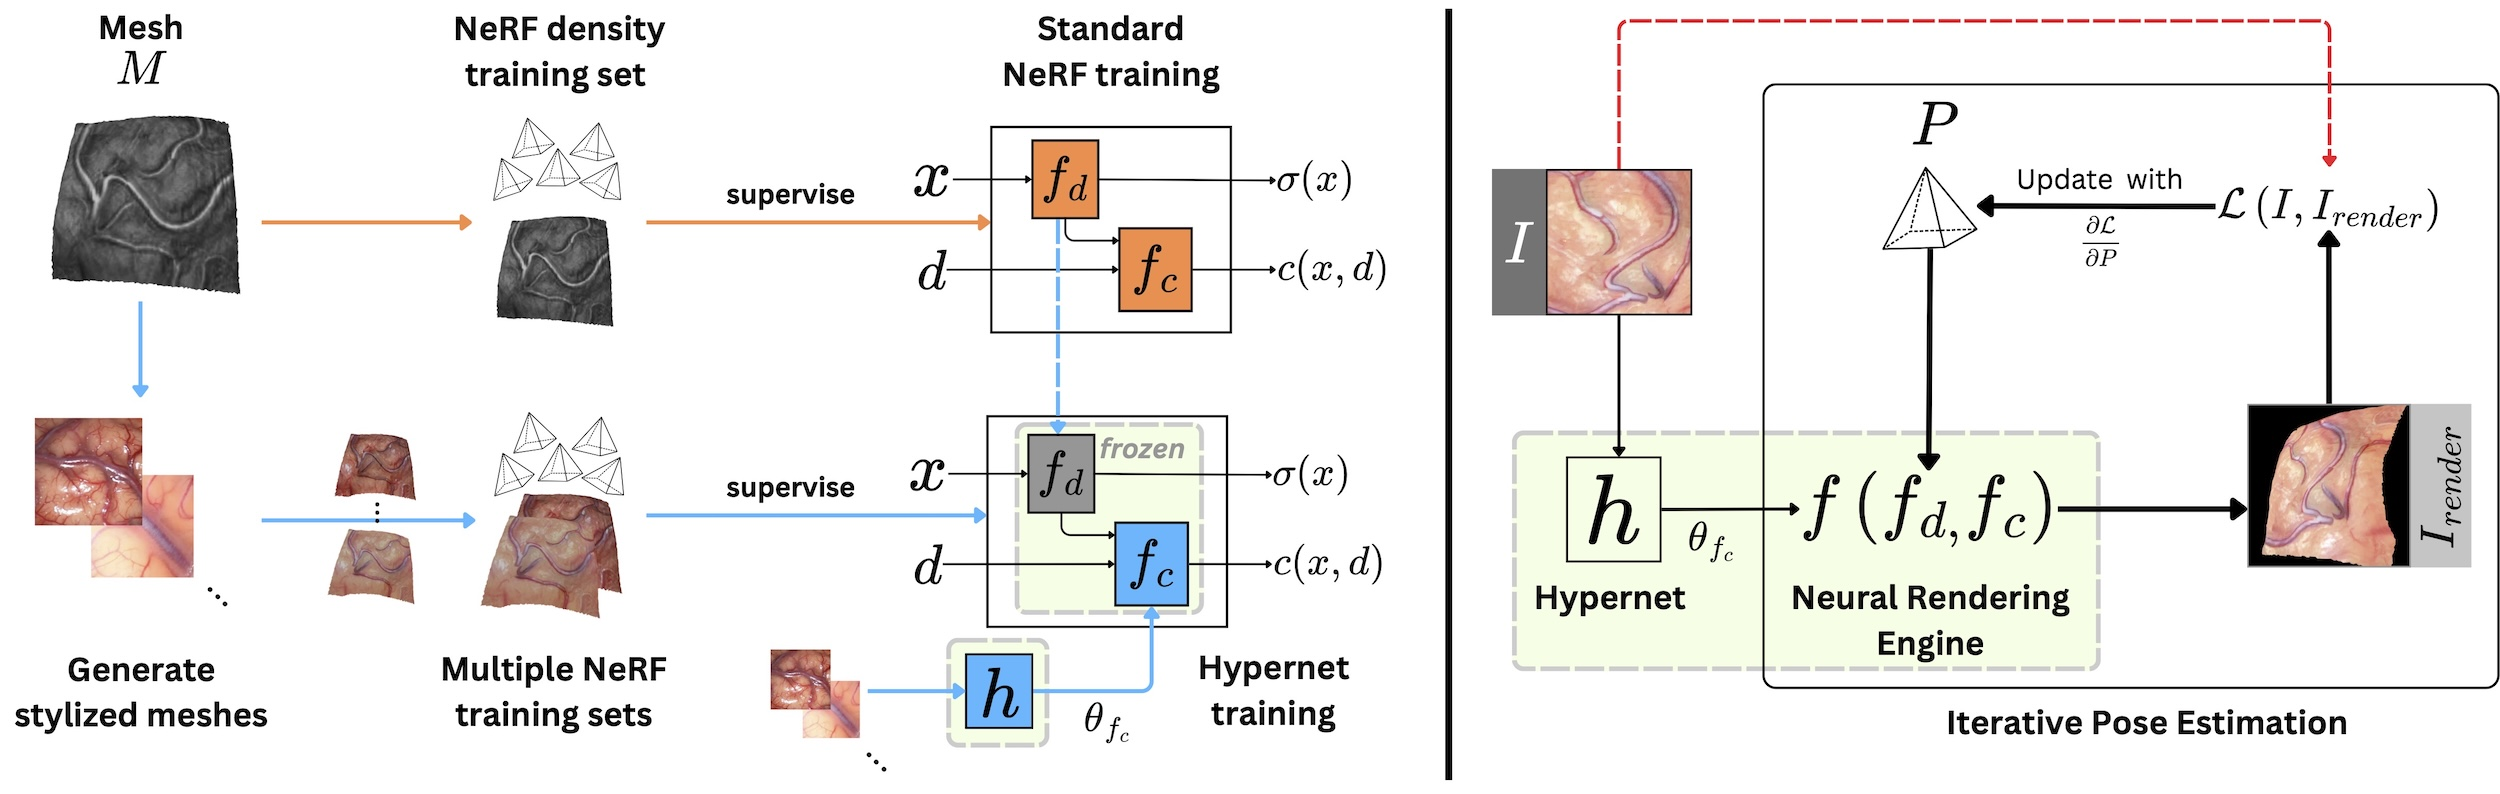
\includegraphics[width=0.9\textwidth]{figures/pipeline.jpg}
  \caption{Overview of the NeRF-based intraoperative registration approach. The method involves preoperative training of a NeRF model on MRI data, followed by intraoperative optimization of camera pose parameters to match the target surgical image.\parencite{fehrentz2024intraoperative}}
  \label{fig:overview}
\end{figure}

% add padding to the figure
\vspace{1cm}

The registration process consists of two main phases:

\begin{enumerate}
    \item \textbf{Preoperative Phase}: A NeRF model is trained using preoperative MRI data to create an implicit representation of the brain's structure.
    
    \item \textbf{Intraoperative Phase}: During surgery, the pre-trained NeRF is used as a differentiable rendering engine. Given a target intraoperative image, the camera pose (6 degrees of freedom) is optimized through a gradient-based approach to match the rendered view with the target image.
\end{enumerate}

\section{Implementation Framework}

One of the primary contributions of this thesis is the development of a flexible, model-agnostic implementation of neural registration built on the nerfstudio framework. Unlike previous implementations that were tied to specific NeRF variants, the proposed framework allows for seamless integration of different NeRF architectures and loss functions.

\subsection{Nerfstudio Integration}

The implementation leverages the nerfstudio framework to ensure flexibility and compatibility with various NeRF architectures. The key components include:

\begin{itemize}
    \item \textbf{Model Agnosticism}: The implementation works with multiple NeRF variants, including the original NeRF \parencite{mildenhall2020nerf}, Instant-NGP \parencite{muller2022instant}, and Nerfacto \parencite{Tancik_2023}, enabling evaluation of different architectures' impact on registration performance.
    
    \item \textbf{Registration Optimizer}: A dedicated optimizer module (the \texttt{iNeRFOptimizerBatchedFD} class) that handles camera pose optimization, loss computation, and experiment tracking.
    
    \item \textbf{Pluggable Loss Functions}: A modular interface for different loss functions, enabling systematic comparison of various similarity metrics.
\end{itemize}

The advantages of this implementation over previous approaches include:
\begin{itemize}
    \item Easy customization of loss functions without modifying the core registration algorithm
    \item Compatibility with nerfstudio's pre-trained models
    \item Integration capabilities with hypernetwork-based appearance adaptation
    \item Comprehensive experiment tracking and visualization
\end{itemize}

\subsection{Finite Difference Optimization}

A notable technical aspect of the implementation is the use of finite difference methods for gradient computation. During development, challenges were encountered with the gradient flow being disconnected in the computational graph when using standard backpropagation. To overcome this limitation while preserving the original concept, a batched finite difference approach for computing gradients was implemented:

\begin{algorithm}[H]
\caption{Batched Finite Difference Gradient Computation}
\begin{algorithmic}[1]
\State \textbf{Input:} Current pose parameters $\theta$, small perturbation $\epsilon$, batch size $B$
\State \textbf{Output:} Gradient $\nabla_{\theta} L$
\State $L_{\text{original}}, \_ \gets \text{ComputeLoss}(\theta)$ \Comment{Compute loss at current pose}
\State $\nabla_{\theta} L \gets \mathbf{0}$ \Comment{Initialize gradient}
\State $\text{coords} \gets \{(i,j) \text{ for all elements } \theta_{i,j} \text{ in } \theta\}$ \Comment{All parameter coordinates}
\For{batch\_start $= 0$ to $|\text{coords}|$ step $B$}
    \State batch\_coords $\gets \text{coords[batch\_start:batch\_start}+B]$
    \State batch\_poses $\gets [\:]$ \Comment{Initialize batch of perturbed poses}
    \For{$(i,j)$ in batch\_coords}
        \State $\theta' \gets \theta$
        \State $\theta'_{i,j} \gets \theta'_{i,j} + \epsilon$ \Comment{Perturb single parameter}
        \State Add $\theta'$ to batch\_poses
    \EndFor
    \State batch\_losses $\gets \text{ComputeBatchLosses(batch\_poses)}$
    \For{idx, $(i,j)$ in enumerate(batch\_coords)}
        \State $\nabla_{\theta_{i,j}} L \gets \frac{\text{batch\_losses[idx]} - L_{\text{original}}}{\epsilon}$ \Comment{Estimate gradient}
    \EndFor
\EndFor
\State \Return $\nabla_{\theta} L$
\end{algorithmic}
\end{algorithm}

This approach offers several advantages:
\begin{itemize}
    \item Robustness to disconnected gradients in the computational graph
    \item Efficient batch processing that significantly reduces computation time
    \item Compatibility with any NeRF model regardless of internal architecture
\end{itemize}

\section{Neural Registration Algorithm}

The complete neural registration algorithm using the implemented framework is presented below:

\begin{algorithm}[H]
\caption{NeRF-based Registration with Customizable Loss Functions}
\begin{algorithmic}[1]
\State \textbf{Input:} Pre-trained NeRF model $\mathcal{N}$, target image $I_{target}$, initial pose $\xi_0$, loss function $\mathcal{L}$, learning rate $\alpha$, number of iterations $T$
\State \textbf{Output:} Optimized camera pose $\hat{\xi}$
\State Initialize pose parameters $\xi \gets \xi_0$
\State Initialize optimizer with pose parameters and learning rate $\alpha$
\State best\_loss $\gets \infty$, best\_pose $\gets \xi_0$
\For{$t = 1$ to $T$}
    \State Compute gradient $\nabla_{\xi} \mathcal{L}$ using batched finite differences:
    \State \hspace{\algorithmicindent} $L_{original}, I_{rendered} \gets \text{ComputeLoss}(\xi)$ \Comment{Forward pass with current pose}
    \State \hspace{\algorithmicindent} $\nabla_{\xi} \mathcal{L} \gets \text{BatchedFiniteDifference}(\xi, L_{original})$
    \State Update pose parameters: $\xi \gets \xi - \alpha \cdot \nabla_{\xi} \mathcal{L}$ \Comment{Gradient descent step}
    \If{$L_{original} < \text{best\_loss}$}
        \State best\_loss $\gets L_{original}$
        \State best\_pose $\gets \xi$
    \EndIf
    \If{$t \bmod \text{visualize\_interval} = 0$}
        \State Visualize current alignment between $I_{target}$ and $I_{rendered}$
    \EndIf
\EndFor
\State \Return best\_pose
\end{algorithmic}
\end{algorithm}

The rendered image $I_{rendered}$ is generated by passing the current camera pose $\xi$ to the pre-trained NeRF model, which produces an RGB prediction. The loss $\mathcal{L}(I_{target}, I_{rendered})$ measures the dissimilarity between the target and rendered images using the selected loss function.

\subsection{Camera Pose Representation}

The camera pose is represented as a 3×4 transformation matrix with the following structure:
\begin{equation}
\xi = \begin{bmatrix} 
R_{11} & R_{12} & R_{13} & t_x \\
R_{21} & R_{22} & R_{23} & t_y \\
R_{31} & R_{32} & R_{33} & t_z
\end{bmatrix}
\end{equation}

where $R$ represents the 3×3 rotation matrix and $t$ represents the translation vector. This 3×4 matrix is converted to the appropriate camera representation using the nerfstudio Camera class during rendering.

\section{Loss Functions for NeRF-Based Registration}\label{section:loss_functions}


The effectiveness of NeRF-based registration fundamentally depends on the choice of loss function, which serves as the mathematical backbone guiding pose optimization. Loss functions quantify the dissimilarity between rendered and target images, effectively creating the optimization landscape that determines convergence behavior and registration accuracy. This section provides a comprehensive analysis of five distinct loss functions (L1, L2, Structural Similarity Index, Normalized Cross-Correlation, and Mutual Information) in the context of intraoperative neural registration. We examine their mathematical formulations, implementation considerations, and comparative performance to understand how different similarity metrics affect registration precision, convergence speed, and robustness to initialization variations. Our systematic evaluation reveals important insights into selecting appropriate loss functions for specific neural registration scenarios, particularly in neurosurgical applications where alignment accuracy directly impacts surgical outcomes.
\subsection{Role of Loss Functions in Registration}

In the context of intraoperative registration using Neural Radiance Fields, the loss function serves two primary purposes:

\begin{enumerate}
    \item \textbf{Similarity Measurement}: It quantifies the similarity between the target intraoperative image and the rendered image from the NeRF model, guiding the optimization process toward better alignment.
    
    \item \textbf{Gradient Provision}: It provides gradients with respect to camera pose parameters, enabling optimization of the camera pose.
\end{enumerate}

\subsection{Implemented Loss Functions}

This section details the loss functions implemented and evaluated in this thesis. Further implementation details can be found in Appendix~\ref{appendix:implementation}. 

\subsubsection{L1 Loss}

The L1 loss, or mean absolute error, calculates the absolute difference between pixel values:

\begin{equation}
\mathcal{L}_{L1}(I_1, I_2) = \frac{1}{N} \sum_{i=1}^{N} |I_1(i) - I_2(i)|
\end{equation}

where $N$ is the number of pixels in the images.

Key characteristics of L1 loss include:
\begin{itemize}
    \item Less sensitivity to outliers compared to L2 loss
    \item Linear behavior that can lead to faster convergence in some cases
    \item Simple gradients that are constant with respect to the error magnitude
\end{itemize}

\subsubsection{L2 Loss}

The L2 loss, or mean squared error (MSE), is the standard baseline approach:

\begin{equation}
\mathcal{L}_{L2}(I_1, I_2) = \frac{1}{N} \sum_{i=1}^{N} (I_1(i) - I_2(i))^2
\end{equation}

Key characteristics of L2 loss include:
\begin{itemize}
    \item Quadratic penalization of large errors
    \item Gradients that scale with the magnitude of the error
    \item Sensitivity to outliers
\end{itemize}

\subsubsection{Structural Similarity Index Loss}

The Structural Similarity Index Measure (SSIM) captures structural information in images:

\begin{equation}
\text{SSIM}(x, y) = \frac{(2\mu_x\mu_y + C_1)(2\sigma_{xy} + C_2)}{(\mu_x^2 + \mu_y^2 + C_1)(\sigma_x^2 + \sigma_y^2 + C_2)}
\end{equation}

The SSIM loss is then defined as:
\begin{equation}
\mathcal{L}_{\text{SSIM}}(I_1, I_2) = 1 - \text{SSIM}(I_1, I_2)
\end{equation}

Key characteristics of SSIM loss include:
\begin{itemize}
    \item Focus on structural information rather than pixel-wise differences
    \item Invariance to certain local transformations
    \item Better correlation with human visual perception
\end{itemize}

\subsubsection{Normalized Cross-Correlation (NCC)}

Normalized Cross-Correlation measures the linear relationship between two images while being invariant to linear intensity transformations:

\begin{equation}
\text{NCC}(I_1, I_2) = \frac{\sum_{i=1}^{N} (I_1(i) - \bar{I}_1)(I_2(i) - \bar{I}_2)}{\sqrt{\sum_{i=1}^{N} (I_1(i) - \bar{I}_1)^2 \sum_{i=1}^{N} (I_2(i) - \bar{I}_2)^2}}
\end{equation}

The NCC loss is then defined as:
\begin{equation}
\mathcal{L}_{\text{NCC}}(I_1, I_2) = 1 - \text{NCC}(I_1, I_2)
\end{equation}

Key characteristics of NCC loss include:
\begin{itemize}
    \item Invariance to linear intensity transformations
    \item Robustness to global illumination changes
    \item Effectiveness for cross-modal registration tasks
\end{itemize}

\subsubsection{Mutual Information (MI)}

Mutual Information quantifies the statistical dependence between two random variables:

\begin{equation}
\text{MI}(I_1, I_2) = \sum_{i,j} p_{I_1,I_2}(i,j) \log\left(\frac{p_{I_1,I_2}(i,j)}{p_{I_1}(i)p_{I_2}(j)}\right)
\end{equation}

The MI loss is defined as:
\begin{equation}
\mathcal{L}_{\text{MI}}(I_1, I_2) = -\text{MI}(I_1, I_2)
\end{equation}

Key characteristics of MI loss include:
\begin{itemize}
    \item Ability to capture complex, non-linear relationships between image intensities
    \item Suitability for cross-modal registration
    \item Robustness to partial overlap between images
\end{itemize}

\section{Experimental Setup}

To rigorously evaluate the impact of different loss functions on Neural Radiance Field (NeRF) based intraoperative registration, a systematic experimental framework was designed with controlled variables and precise measurement protocols.

\subsection{Technical Configuration}

The experiments were conducted with the following specifications to ensure fair and consistent comparison across loss functions:
\begin{itemize}
    \item \textbf{Optimization Parameters}: Fixed at 50 iterations across all experiments to standardize convergence conditions
    \item \textbf{Optimization Algorithm}: AdamW optimizer with a learning rate of 0.01, chosen for its adaptive momentum properties and weight decay regularization
    \item \textbf{Gradient Computation}: Finite difference approximation with epsilon value of $1 \times 10^{-4}$ for gradient stability
    \item \textbf{Experimental Runs}: 10 different initial camera poses per loss function to ensure statistical significance and account for local optimization challenges
    \item \textbf{Target Consistency}: Identical target image used across all experiments to eliminate target-specific biases
    \item \textbf{Data Source Control}: Both target images and rendered views sourced from the same pre-trained NeRF model to eliminate variations due to domain gaps or rendering inconsistencies
    \item \textbf{Batch Size}: Set at 12 for finite difference calculations to optimize the trade-off between memory usage and computational efficiency
\end{itemize}

\subsection{Loss Functions}

As previously introduced in Section~\ref{section:loss_functions}, five distinct loss functions were systematically evaluated to compare their performance in NeRF-based registration:

\begin{itemize}
    \item \textbf{L1 Loss (Mean Absolute Error)}
    
    \item \textbf{L2 Loss (Mean Squared Error)}
    
    \item \textbf{Structural Similarity Index Loss (SSIM)}
    
    \item \textbf{Normalized Cross-Correlation (NCC)}
    
    \item \textbf{Mutual Information Loss (MI)}
\end{itemize}

Each loss function was selected for its unique properties and potential advantages in medical image registration: L1 and L2 for their direct intensity comparisons with different sensitivity to outliers; SSIM for its emphasis on structural information; NCC for its robustness to linear intensity variations; and MI for its capacity to handle multi-modal image alignment.

\subsection{Evaluation Metrics}

Registration performance was comprehensively evaluated using the following quantitative and qualitative metrics:

\begin{itemize}
    \item \textbf{Convergence Efficiency}: Measured by identifying the iteration at which the optimal loss value was achieved, providing insight into each loss function's optimization trajectory
    
    \item \textbf{Computational Performance}: Total time required for the complete optimization process, broken down into component stages including forward passes, gradient calculations, and parameter updates
    
    \item \textbf{Registration Accuracy}: Quantified through:
    \begin{itemize}
        \item Final loss value achieved
        \item Pixel-wise alignment between registered and target images
        \item Visual overlay assessment by superimposing the registered image on the target with 50\% transparency
    \end{itemize}
    
    \item \textbf{Optimization Stability}: Analyzed through:
    \begin{itemize}
        \item Loss curve smoothness and monotonicity
        \item Variance in pose parameter updates across iterations
        \item Resistance to local minima in the optimization landscape
    \end{itemize}
    
    \item \textbf{Robustness to NeRF Artifacts}: Qualitative assessment of how each loss function performs in the presence of rendering inconsistencies
\end{itemize}

\subsection{Experiment Tracking and Data Collection}

A comprehensive tracking framework was implemented to capture all relevant experimental data:

\begin{itemize}
    \item \textbf{Parameter Trajectory}: Complete camera pose transformation matrix recorded at each iteration
    
    \item \textbf{Loss Dynamics}: Full loss history with values captured after each optimization step
    
    \item \textbf{Visual Documentation}: 
    \begin{itemize}
        \item Rendered images saved at regular intervals (every 10 iterations)
        \item Side-by-side visualizations of target and current rendered images
        \item Progressive alignment overlays to visually track registration improvement
    \end{itemize}
    
    \item \textbf{Performance Profiling}:
    \begin{itemize}
        \item Per-iteration timing statistics
        \item Computational resource utilization
        \item Batch processing efficiency metrics for finite difference calculations
    \end{itemize}
    
    \item \textbf{Metadata Management}: Structured JSON tracking files containing complete experimental parameters, iteration history, and final results for reproducibility and further analysis
\end{itemize}

All experimental data was systematically organized in a standardized directory structure to facilitate comparative analysis and ensure reproducibility of results.

\section{Summary}

This chapter has presented a comprehensive methodology for enhancing intraoperative registration using Neural Radiance Fields. The key contributions include:

\begin{enumerate}
    \item Development of a flexible, model-agnostic implementation of neural registration integrated with the nerfstudio framework
    \item Implementation of a batched finite difference approach for robust gradient computation
    \item Systematic evaluation of multiple loss functions (L1, L2, SSIM, NCC, MI) for NeRF-based registration
    \item A controlled experimental setup for fair comparison of different approaches
\end{enumerate}

The results of these experiments are presented and analyzed in Chapter~\ref{chapter:results}.  %prev 03-05 combined
%% !TeX root = ../main.tex

\chapter{Loss Functions for NeRF-Based Registration}\label{chapter:loss_functions}

This chapter provides a detailed analysis of various loss functions and their application to NeRF-based intraoperative registration. We investigate how different similarity measures affect registration accuracy, convergence speed, and robustness to cross-modal appearance variations. The loss function is a critical component of the registration framework, as it defines the optimization objective that guides the camera pose estimation process.

\section{Role of Loss Functions in Registration}

In the context of intraoperative registration using Neural Radiance Fields, the loss function serves two primary purposes:

\begin{enumerate}
    \item \textbf{Similarity Measurement}: It quantifies the similarity between the target intraoperative image and the rendered image from the NeRF model. This measure guides the optimization process toward better alignment.
    
    \item \textbf{Gradient Provision}: It provides gradients with respect to camera pose parameters, enabling backpropagation-based optimization of the camera pose.
\end{enumerate}

The effectiveness of a loss function depends on its ability to handle cross-modal differences between preoperative MRI-derived renderings and intraoperative camera images. Different loss functions have varying sensitivities to factors such as:

\begin{itemize}
    \item Intensity scaling and bias
    \item Local contrast variations
    \item Texture and high-frequency details
    \item Noise and outliers
    \item Incomplete overlap between images
\end{itemize}

\section{L2 Loss: Baseline Approach}

The L2 loss, or mean squared error (MSE), is commonly used in registration tasks and serves as our baseline approach. For two images $I_1$ and $I_2$, the L2 loss is defined as:

\begin{equation}
    \mathcal{L}_{\text{L2}}(I_1, I_2) = \frac{1}{N} \sum_{i=1}^{N} (I_1(i) - I_2(i))^2
\end{equation}

where $N$ is the number of pixels in the images.

\subsection{Implementation Details}

Our implementation of the L2 loss includes the following components:

\begin{itemize}
    \item \textbf{Normalization}: To improve robustness to global intensity variations, we normalize the images to have zero mean and unit standard deviation before computing the loss.
    
    \item \textbf{Channel Weighting}: We allow for different weights to be assigned to different color channels, potentially prioritizing channels with more relevant information.
    
    \item \textbf{Differentiability}: The L2 loss is fully differentiable with respect to the input images, enabling end-to-end gradient flow from the loss to the camera pose parameters.
\end{itemize}

\subsection{Advantages and Limitations}

The L2 loss offers several advantages:
\begin{itemize}
    \item Simplicity and computational efficiency
    \item Well-defined gradients for optimization
    \item Direct interpretation as the Euclidean distance in pixel space
\end{itemize}

However, it also has significant limitations for cross-modal registration:
\begin{itemize}
    \item High sensitivity to intensity variations and outliers
    \item Assumption of direct correspondence between pixel intensities across modalities
    \item Limited capture range, potentially leading to local minima
\end{itemize}

\section{Normalized Cross-Correlation (NCC)}

Normalized Cross-Correlation measures the linear relationship between two images while being invariant to linear intensity transformations. The NCC loss is defined as:

\begin{equation}
    \mathcal{L}_{\text{NCC}}(I_1, I_2) = -\frac{\sum_{i=1}^{N} (I_1(i) - \bar{I}_1)(I_2(i) - \bar{I}_2)}{\sqrt{\sum_{i=1}^{N} (I_1(i) - \bar{I}_1)^2 \sum_{i=1}^{N} (I_2(i) - \bar{I}_2)^2}}
\end{equation}

where $\bar{I}_1$ and $\bar{I}_2$ are the mean intensities of the respective images. The negative sign is used because we're minimizing the loss, while NCC itself is a similarity measure that should be maximized.

\subsection{Implementation Details}

Our implementation of NCC includes several enhancements:

\begin{itemize}
    \item \textbf{Local NCC}: We implement both global NCC (computed over the entire image) and local NCC (computed over small patches), which can better handle local intensity variations.
    
    \item \textbf{Multi-scale NCC}: We compute NCC at multiple scales to capture both fine details and broader structures.
    
    \item \textbf{Regularization}: A small constant $\epsilon$ is added to the denominator to ensure numerical stability:
    \begin{equation}
        \mathcal{L}_{\text{NCC}}(I_1, I_2) = -\frac{\sum_{i=1}^{N} (I_1(i) - \bar{I}_1)(I_2(i) - \bar{I}_2)}{\sqrt{(\sum_{i=1}^{N} (I_1(i) - \bar{I}_1)^2 + \epsilon)(\sum_{i=1}^{N} (I_2(i) - \bar{I}_2)^2 + \epsilon)}}
    \end{equation}
\end{itemize}

\subsection{Advantages and Limitations}

NCC offers several advantages over L2 loss for cross-modal registration:
\begin{itemize}
    \item Invariance to linear intensity transformations (scaling and bias)
    \item Better robustness to global illumination changes
    \item Often more effective for cross-modal registration tasks \parencite{nccreg}
\end{itemize}

However, NCC also has limitations:
\begin{itemize}
    \item Only captures linear relationships between images
    \item May be less effective when the relationship between modalities is non-linear
    \item Computationally more expensive than L2 loss
\end{itemize}

\section{Mutual Information (MI)}

Mutual Information is a statistical measure from information theory that quantifies the mutual dependence between two random variables. In the context of image registration, MI measures how much information one image provides about another, making it particularly suitable for cross-modal registration where the relationship between intensities is complex and non-linear.

The MI loss is defined as:

\begin{equation}
    \mathcal{L}_{\text{MI}}(I_1, I_2) = -\sum_{i,j} p_{I_1,I_2}(i,j) \log\left(\frac{p_{I_1,I_2}(i,j)}{p_{I_1}(i)p_{I_2}(j)}\right)
\end{equation}

where $p_{I_1,I_2}$ is the joint probability distribution of intensities in images $I_1$ and $I_2$, and $p_{I_1}$ and $p_{I_2}$ are their marginal distributions. As with NCC, the negative sign is used to convert the similarity measure to a loss function for minimization.

\subsection{Implementation Details}

Implementing MI for differentiable optimization presents several challenges, which we address through the following approaches:

\begin{itemize}
    \item \textbf{Histogram Computation}: We compute joint and marginal histograms of image intensities using differentiable binning functions based on B-splines.
    
    \item \textbf{Parzen Window Estimation}: To create continuous, differentiable probability distributions, we employ Parzen window estimation with Gaussian kernels.
    
    \item \textbf{Normalized MI}: We implement normalized mutual information (NMI) as an alternative formulation:
    \begin{equation}
        \mathcal{L}_{\text{NMI}}(I_1, I_2) = -\frac{H(I_1) + H(I_2)}{H(I_1, I_2)}
    \end{equation}
    where $H(I_1)$ and $H(I_2)$ are the marginal entropies, and $H(I_1, I_2)$ is the joint entropy.
\end{itemize}

\subsection{Advantages and Limitations}

MI offers significant advantages for cross-modal registration:
\begin{itemize}
    \item Captures complex, non-linear relationships between image intensities
    \item Well-suited for cross-modal registration tasks \parencite{mi2003}
    \item Robust to partial overlap between images
\end{itemize}

However, MI also has limitations:
\begin{itemize}
    \item Computationally expensive to calculate
    \item Can have complex gradient behavior
    \item May have a smaller capture range than other metrics
    \item Requires careful implementation to ensure differentiability
\end{itemize}

\section{Weighted and Masked L2 Loss}

The standard L2 loss treats all pixels equally, which may not be optimal for registration tasks where certain regions contain more relevant information than others. We extend the L2 loss with weighting and masking mechanisms to address this limitation.

\subsection{Spatially Weighted L2 Loss}

The spatially weighted L2 loss assigns different importance to different regions of the image:

\begin{equation}
    \mathcal{L}_{\text{wL2}}(I_1, I_2) = \frac{1}{N} \sum_{i=1}^{N} w(i) (I_1(i) - I_2(i))^2
\end{equation}

where $w(i)$ is a weight value for pixel $i$. We explore several strategies for determining these weights:

\begin{itemize}
    \item \textbf{Gradient-based weighting}: Assigning higher weights to regions with high gradient magnitude, which typically correspond to edges and features.
    
    \item \textbf{Vessel-enhanced weighting}: Using vessel enhancement filters to prioritize vascular structures, which are prominent landmarks in brain surface images.
    
    \item \textbf{Saliency-based weighting}: Employing visual saliency models to identify regions that are perceptually important.
\end{itemize}

\subsection{Binary Masking}

Binary masking is a special case of weighting where $w(i) \in \{0, 1\}$. This approach excludes certain regions from the loss calculation entirely:

\begin{equation}
    \mathcal{L}_{\text{mL2}}(I_1, I_2) = \frac{1}{\sum_{i=1}^{N} m(i)} \sum_{i=1}^{N} m(i) (I_1(i) - I_2(i))^2
\end{equation}

where $m(i) \in \{0, 1\}$ is a binary mask. Binary masking is particularly useful for:

\begin{itemize}
    \item Excluding background regions
    \item Focusing on regions of interest (e.g., the exposed brain surface)
    \item Handling partial overlap between the preoperative model and intraoperative view
\end{itemize}

\subsection{Implementation Details}

Our implementation of weighted and masked L2 loss includes:

\begin{itemize}
    \item \textbf{Automatic mask generation}: Algorithms for automatically generating masks based on image content.
    
    \item \textbf{Differentiable weighting}: Ensuring that the weighting mechanism preserves differentiability for gradient-based optimization.
    
    \item \textbf{Adaptive weighting}: Dynamically adjusting weights based on the current registration state.
\end{itemize}

\section{Combined Loss Functions}

Different loss functions capture different aspects of image similarity. To leverage the complementary strengths of various metrics, we explore combinations of loss functions:

\begin{equation}
    \mathcal{L}_{\text{combined}} = \alpha \mathcal{L}_1 + \beta \mathcal{L}_2 + \gamma \mathcal{L}_3
\end{equation}

where $\mathcal{L}_1$, $\mathcal{L}_2$, and $\mathcal{L}_3$ are different loss functions, and $\alpha$, $\beta$, and $\gamma$ are weighting coefficients.

\subsection{Adaptive Weighting Strategies}

Instead of fixed weights, we implement adaptive weighting strategies that adjust the contribution of each loss component based on the current registration state:

\begin{itemize}
    \item \textbf{Phase-based weighting}: Using different weights during different phases of the optimization (e.g., coarse-to-fine alignment).
    
    \item \textbf{Confidence-based weighting}: Adjusting weights based on the confidence or reliability of each metric for the current images.
    
    \item \textbf{Gradient-based weighting}: Weighting loss components based on the magnitude and direction of their gradients to improve convergence.
\end{itemize}

\section{Experimental Evaluation of Loss Functions}

To systematically evaluate the effectiveness of different loss functions for NeRF-based intraoperative registration, we conduct a series of experiments comparing their performance under various conditions.

\subsection{Experimental Setup}

The experiments are designed to test the following aspects:

\begin{itemize}
    \item \textbf{Registration Accuracy}: Ability to achieve accurate alignment measured by pose error and target registration error.
    
    \item \textbf{Convergence Behavior}: Speed of convergence and ability to avoid local minima.
    
    \item \textbf{Robustness to Modality Differences}: Performance when facing differences in appearance between preoperative and intraoperative images.
    
    \item \textbf{Sensitivity to Initialization}: Capture range and dependency on initial pose estimates.
\end{itemize}

\subsection{Results and Analysis}

The detailed results of these experiments are presented in Chapter~\ref{chapter:results}. However, preliminary findings indicate that:

\begin{itemize}
    \item NCC consistently outperforms L2 loss in the presence of intensity variations.
    
    \item MI shows promise for handling complex cross-modal differences but requires careful implementation to ensure stable gradients.
    
    \item Weighted L2 loss with gradient-based or vessel-enhanced weighting significantly improves over standard L2 loss.
    
    \item Combined loss functions can leverage complementary strengths, especially when using adaptive weighting strategies.
\end{itemize}

\section{Summary}

This chapter has presented a comprehensive exploration of various loss functions for NeRF-based intraoperative registration. We have detailed the mathematical formulations, implementation considerations, and theoretical properties of L2 loss, Normalized Cross-Correlation, Mutual Information, and weighted/masked variants. Additionally, we have introduced combined loss functions with adaptive weighting strategies to leverage the complementary strengths of different metrics.

The choice of loss function significantly impacts registration performance, particularly in the challenging context of cross-modal alignment between preoperative MRI-derived renderings and intraoperative camera images. The next chapter will explore another critical aspect of our approach: style transfer techniques for bridging the appearance gap between modalities. 
%% !TeX root = ../main.tex

\chapter{Style Transfer for Cross-Modal Registration}\label{chapter:style_transfer}

This chapter explores the use of style transfer techniques to enhance cross-modal registration between preoperative MRI data and intraoperative optical images. We examine how adapting the appearance of NeRF-rendered images through style transfer can bridge the modality gap and improve registration accuracy. Various style encoding methods and hypernetwork architectures are investigated to determine their effectiveness in the context of neurosurgical registration.

\section{The Cross-Modal Appearance Gap}

One of the fundamental challenges in intraoperative registration is the significant difference in appearance between preoperative MRI data and intraoperative optical images:

\begin{itemize}
    \item \textbf{MRI data} typically presents in grayscale with contrast determined by tissue properties such as T1/T2 relaxation times and proton density.
    
    \item \textbf{Intraoperative optical images} capture the visible surface of the brain with natural color, specular highlights, shadows, and various lighting effects.
\end{itemize}

This appearance gap complicates the registration process, as conventional similarity metrics may struggle to establish correspondence between such visually different representations. Style transfer techniques offer a promising approach to address this challenge by transforming the appearance of NeRF-rendered images to match the visual characteristics of intraoperative images while preserving the underlying anatomical structure.

\section{Hypernetwork-Based Style Control}

Building on the approach introduced by \textcite{fehrentz2024intraoperative}, we employ hypernetworks as a mechanism for controlling the appearance of NeRF renderings. A hypernetwork is a neural network that generates parameters for another neural network (in this case, the NeRF model) based on conditioning information (in this case, style descriptors).

\subsection{Architecture Overview}

Our hypernetwork-based style control system consists of three main components:

\begin{enumerate}
    \item \textbf{Style Encoder}: Extracts style information from reference images or generates style codes from abstract style specifications.
    
    \item \textbf{Hypernetwork}: Generates parameters for a subset of the NeRF model based on the encoded style.
    
    \item \textbf{Parameter Integration}: Incorporates the generated parameters into the NeRF model to influence its rendering appearance.
\end{enumerate}

Figure~\ref{fig:hypernetwork} illustrates this architecture.

% Placeholder for hypernetwork figure
\begin{figure}[htpb]
  \centering
  % Add actual figure in the implementation
  \caption{Architecture of the hypernetwork-based style control system. The style encoder extracts style information from reference images, which the hypernetwork transforms into parameters for the NeRF model, controlling the appearance of rendered images.}
  \label{fig:hypernetwork}
\end{figure}

\subsection{Hypernetwork Design}

We explore several design choices for the hypernetwork:

\begin{itemize}
    \item \textbf{Network Depth and Width}: We compare hypernetworks of different sizes to balance expressiveness and computational efficiency.
    
    \item \textbf{Parameter Generation Scope}: We investigate which NeRF model parameters should be generated by the hypernetwork to effectively control appearance while preserving structure.
    
    \item \textbf{Conditioning Mechanisms}: We experiment with different ways of incorporating style information, including feature concatenation, adaptive instance normalization (AdaIN), and modulation-based approaches.
\end{itemize}

Our findings indicate that generating parameters for the color prediction layers while keeping the density prediction layers fixed provides the best balance between appearance control and structural preservation.

\section{Style Encoding Methods}

A critical aspect of our approach is how style information is encoded and represented. We explore various methods for extracting and encoding style information from reference images:

\subsection{Y'UV Color Space Encoding}

The Y'UV color space separates luminance (Y') from chrominance (U, V), allowing for more intuitive control over color characteristics. Our Y'UV encoding approach includes:

\begin{itemize}
    \item \textbf{Color Space Transformation}: Converting RGB images to Y'UV space.
    
    \item \textbf{Statistical Moments}: Capturing the mean and variance of each channel across the image.
    
    \item \textbf{Histogram Matching}: Aligning the distributions of Y'UV channels between rendered and target images.
\end{itemize}

This method is particularly effective for handling global color differences while requiring relatively low computational resources.

\subsection{Histogram of Oriented Gradients (HOG)}

HOG features capture the distribution of gradient orientations in local regions of an image, providing information about edge patterns and texture directions. Our HOG-based style encoding includes:

\begin{itemize}
    \item \textbf{Feature Extraction}: Computing HOG features at multiple scales.
    
    \item \textbf{Feature Aggregation}: Pooling HOG descriptors to create a compact style representation.
    
    \item \textbf{Feature Integration}: Incorporating HOG information into the style code.
\end{itemize}

HOG encoding helps preserve edge structures and directional patterns, which are important for registration accuracy, especially in regions with distinct vascular patterns.

\subsection{Texture Features and Gabor Filters}

Texture is a key characteristic that differs between MRI and optical images. We explore texture-based style encoding using:

\begin{itemize}
    \item \textbf{Gabor Filter Banks}: Applying filters at multiple orientations and scales to capture texture patterns.
    
    \item \textbf{Local Binary Patterns (LBP)}: Extracting rotation-invariant texture descriptors.
    
    \item \textbf{Texture Moments}: Computing statistical moments of filter responses to create compact texture representations.
\end{itemize}

These texture features help model the fine-grained appearance differences between imaging modalities, particularly for tissue textures that are not captured by simpler color-based encodings.

\subsection{Edge Detection and Contour Matching}

Edges and contours often represent anatomically meaningful boundaries that are consistent across modalities. Our edge-based encoding includes:

\begin{itemize}
    \item \textbf{Edge Detection}: Applying operators such as Canny, Sobel, or learned edge detectors.
    
    \item \textbf{Contour Extraction}: Identifying continuous contours in both rendered and target images.
    
    \item \textbf{Contour Matching}: Aligning contour representations across modalities.
\end{itemize}

This approach helps preserve anatomical boundaries and structural information during style transfer, which is crucial for accurate registration.

\subsection{Gram Matrix for Style Representation}

Inspired by neural style transfer methods, we investigate the use of Gram matrices to capture style information:

\begin{itemize}
    \item \textbf{Feature Extraction}: Using a pre-trained convolutional neural network to extract features from images.
    
    \item \textbf{Gram Matrix Computation}: Calculating the correlation between features at different channels to create a style representation.
    
    \item \textbf{Multi-layer Representation}: Computing Gram matrices at multiple layers to capture both fine and coarse stylistic elements.
\end{itemize}

Gram matrices effectively capture texture patterns and style information at different scales, providing a rich representation for style transfer.

\subsection{Deep Feature Matching}

We explore the use of features extracted from pre-trained convolutional neural networks (CNNs) for style encoding:

\begin{itemize}
    \item \textbf{Feature Extraction}: Using networks pre-trained on medical imaging or natural image datasets.
    
    \item \textbf{Feature Selection}: Identifying the most relevant features for cross-modal matching.
    
    \item \textbf{Feature Adaptation}: Fine-tuning the feature extraction process for the specific task of neurosurgical image matching.
\end{itemize}

Deep features can capture high-level semantic information that may be consistent across modalities, potentially improving the registration of anatomical structures.

\section{Structural Similarity Preservation}

While adapting appearance, it is crucial to preserve the structural information that is essential for accurate registration. We implement several mechanisms to ensure structural similarity:

\subsection{Structural Similarity Index (SSIM)}

We incorporate the Structural Similarity Index as both an evaluation metric and a loss component to preserve structural information:

\begin{equation}
    \text{SSIM}(x, y) = \frac{(2\mu_x\mu_y + C_1)(2\sigma_{xy} + C_2)}{(\mu_x^2 + \mu_y^2 + C_1)(\sigma_x^2 + \sigma_y^2 + C_2)}
\end{equation}

where $\mu_x$, $\mu_y$ are the means, $\sigma_x$, $\sigma_y$ are the standard deviations, and $\sigma_{xy}$ is the covariance of patches from images $x$ and $y$. The constants $C_1$ and $C_2$ prevent division by zero.

\subsection{Structure-Preserving Constraints}

We implement additional constraints to ensure that style transfer does not alter structural information:

\begin{itemize}
    \item \textbf{Density Preservation}: Keeping the density predictions of the NeRF model fixed while only modifying color predictions.
    
    \item \textbf{Edge Alignment}: Ensuring that edges in the rendered images align with those in the target images, regardless of appearance differences.
    
    \item \textbf{Gradient Consistency}: Maintaining consistent gradient directions between original and style-transferred renderings.
\end{itemize}

\section{Style Optimization during Registration}

During the registration process, we need to simultaneously optimize camera pose and style parameters. We explore different strategies for this joint optimization:

\subsection{Sequential Optimization}

The sequential approach alternates between optimizing style parameters and camera pose:

\begin{enumerate}
    \item \textbf{Style Adaptation Phase}: Fix camera pose and optimize style parameters for a few iterations.
    
    \item \textbf{Pose Optimization Phase}: Fix style parameters and optimize camera pose for a few iterations.
    
    \item \textbf{Repeat}: Continue alternating until convergence.
\end{enumerate}

This approach can help avoid local minima by separating the optimization of appearance and geometry.

\subsection{Joint Optimization}

The joint approach optimizes both style parameters and camera pose simultaneously:

\begin{equation}
    \hat{\xi}, \hat{s} = \arg\min_{\xi, s} \mathcal{L}(I_{\text{target}}, I_{\text{rendered}}(\xi, s))
\end{equation}

This approach is more efficient but requires careful balancing of gradients to prevent one set of parameters from dominating the optimization.

\subsection{Multi-Stage Optimization}

The multi-stage approach breaks the optimization into distinct phases:

\begin{enumerate}
    \item \textbf{Initial Style Adaptation}: Optimize style parameters with a fixed initial pose.
    
    \item \textbf{Coarse Pose Optimization}: Optimize camera pose at a low resolution with fixed style.
    
    \item \textbf{Refinement}: Jointly fine-tune both pose and style at higher resolution.
\end{enumerate}

This approach combines the benefits of sequential and joint optimization while addressing their limitations.

\section{Experimental Evaluation of Style Transfer Methods}

To evaluate the effectiveness of different style encoding methods and optimization strategies, we conduct a series of experiments:

\subsection{Style Transfer Quality Assessment}

We assess the quality of style transfer using both quantitative metrics and qualitative evaluation:

\begin{itemize}
    \item \textbf{Appearance Similarity}: Measures how well the rendered images match the target style.
    
    \item \textbf{Structure Preservation}: Evaluates whether structural information is preserved during style transfer.
    
    \item \textbf{Artifact Analysis}: Examines the presence of artifacts or distortions introduced by style transfer.
\end{itemize}

\subsection{Registration Performance with Style Transfer}

We evaluate how different style transfer methods affect registration performance:

\begin{itemize}
    \item \textbf{Registration Accuracy}: Comparing pose estimation accuracy with and without style transfer.
    
    \item \textbf{Convergence Behavior}: Analyzing how style transfer affects optimization convergence.
    
    \item \textbf{Robustness to Initial Conditions}: Testing registration performance with various initial poses.
\end{itemize}

\subsection{Comparison of Style Encoding Methods}

We compare the performance of different style encoding methods in the context of intraoperative registration:

\begin{itemize}
    \item \textbf{Y'UV vs. HOG vs. Texture Features}: Evaluating which encoding methods work best for different types of images.
    
    \item \textbf{Simple vs. Complex Encodings}: Analyzing the trade-off between computational complexity and performance.
    
    \item \textbf{Single vs. Combined Encodings}: Testing whether combining multiple encoding methods yields better results.
\end{itemize}

\section{Results and Analysis}

The detailed results of our style transfer experiments are presented in Chapter~\ref{chapter:results}. However, preliminary findings indicate that:

\begin{itemize}
    \item Y'UV color space encoding provides effective global color adaptation while being computationally efficient.
    
    \item HOG and texture features improve registration in regions with distinctive vessel patterns.
    
    \item Gram matrices capture rich stylistic information but require more computational resources.
    
    \item Multi-stage optimization strategy generally outperforms both sequential and joint optimization approaches.
    
    \item Style transfer significantly improves registration accuracy in cases with substantial appearance differences between preoperative and intraoperative images.
\end{itemize}

\section{Summary}

This chapter has presented a comprehensive exploration of style transfer techniques for enhancing cross-modal registration using Neural Radiance Fields. We have detailed various style encoding methods, from simple color space transformations to complex deep feature representations, and analyzed their effectiveness in bridging the appearance gap between preoperative MRI data and intraoperative optical images.

The integration of style transfer with NeRF-based registration through hypernetworks provides a powerful framework for adapting appearance while preserving structural information. Our experimental results suggest that this approach can significantly improve registration accuracy in the challenging context of neurosurgical navigation.

The next chapter will describe the experimental setup used to evaluate both the loss functions discussed in Chapter~\ref{chapter:loss_functions} and the style transfer techniques presented in this chapter. 
%\input{chapters/03-05_combined}
% \input{chapters/04_experiments}
% !TeX root = ../main.tex

\chapter{Results}\label{chapter:results}

This chapter presents the experimental results of our investigation into enhancing intraoperative registration with Neural Radiance Fields through different loss functions. We begin with a description of our nerfstudio-based implementation, followed by a comprehensive evaluation of different loss functions and their impact on registration performance.

\section{NeRF-Based Registration Implementation}

One of the primary contributions of this work is the development of a nerfstudio-based implementation of neural registration that is agnostic to the specific NeRF model architecture (e.g., vanilla NeRF, InstantNGP). This implementation leverages finite differences to compute gradients and provides a flexible framework for experimenting with different loss functions.

\subsection{Optimization Strategy}

Our implementation follows an inverse neural rendering approach inspired by iNeRF \parencite{yen2020inerf}. The key steps in our optimization strategy are as follows:

\begin{enumerate}
    \item Start with an initial camera pose in 3D NeRF space, represented as a transformation matrix.
    
    \item Render a snapshot from the pre-trained NeRF at the current pose.
    
    \item Calculate the error between the rendered image and the target image using the selected loss function.
    
    \item Update the camera pose through optimization to minimize this error.
    
    \item Repeat steps 2-4 until convergence or a maximum number of iterations is reached.
\end{enumerate}

To overcome challenges with gradient flow disconnection in the rendering pipeline, we implemented a finite differences approach for gradient computation. This approach, while computationally more intensive than direct backpropagation, provides stable and reliable gradients for pose optimization.

\section{Loss Function Evaluation}

We evaluated the performance of five different loss functions in the context of NeRF-based registration:

\begin{itemize}
    \item L1 Loss (Mean Absolute Error)
    \item L2 Loss (Mean Squared Error)
    \item Structural Similarity Index Loss (SSIM)
    \item Normalized Cross-Correlation Loss (NCC)
    \item Mutual Information Loss (MI)
\end{itemize}

Our evaluation focused on convergence behavior, stability, and final registration accuracy across multiple starting positions.

\subsection{Experimental Setup}

To ensure controlled and reproducible results, we established the following experimental setup:

\begin{itemize}
    \item All experiments were limited to 50 iterations
    \item AdamW optimizer with a learning rate of 0.01
    \item 10 different starting points with the same target image
    \item Both target and rendered images sourced from the same NeRF model
    \item Batch size of 12 for finite differences gradient computation
\end{itemize}

\subsection{Convergence Behavior}

Table~\ref{tab:loss_convergence} summarizes the average convergence performance of different loss functions in our experiments.

\begin{table}[htpb]
  \caption[Convergence performance of different loss functions]{Average convergence performance of different loss functions.}\label{tab:loss_convergence}
  \centering
  \begin{tabular}{l c c}
    \toprule
      Loss Function & Average Best Loss Iteration & Average Time Elapsed (s) \\
    \midrule
      L1 & 39 & 621 \\
      L2 & 47 & 624 \\
      Structural Similarity Index & 49 & 626 \\
      Normalized Cross-Correlation & 44 & 621 \\
      Mutual Information & 42 & 621 \\
    \bottomrule
  \end{tabular}
\end{table}

Our results indicate that L1 loss converges more quickly on average compared to other loss functions, reaching its best loss value around iteration 39. In contrast, SSIM requires almost the full 50 iterations before converging to its best value.

Figure~\ref{fig:loss_convergence} illustrates the typical convergence behavior of different loss functions during the registration optimization process.

\begin{figure}[htpb]
  \centering
  % Add actual figure in the implementation
  \caption[Convergence behavior of different loss functions]{Convergence behavior of different loss functions during registration optimization. The plot shows the evolution of loss as a function of optimization iterations.}
  \label{fig:loss_convergence}
\end{figure}

\subsection{Qualitative Analysis}

Our qualitative analysis of the optimization trajectories revealed several interesting patterns:

\begin{itemize}
    \item L1 and L2 losses tend to follow smoother, more direct paths during optimization, with L1 generally converging faster.
    
    \item Mutual Information and Normalized Cross-Correlation losses exhibit more "exploratory" behavior in early iterations, with more pronounced oscillations in the optimization path.
    
    \item SSIM demonstrates slower initial progress but continues to improve throughout the optimization process.
    
    \item MI and NCC appear to be more robust to NeRF rendering artifacts, potentially making them more suitable for cross-modal scenarios.
\end{itemize}

\subsection{Registration Accuracy and Stability}

While all loss functions eventually achieved visually satisfactory registration results, our observations suggest differences in their stability and robustness:

\begin{itemize}
    \item L1 loss provides the fastest convergence while maintaining good stability.
    
    \item MI and NCC show greater resilience to local optima, potentially offering advantages in real-world scenarios with imperfect NeRF representations.
    
    \item SSIM focuses more on structural alignment at multiple scales, which may be beneficial for preserving anatomical structure correspondence.
\end{itemize}

\section{L1 Loss Performance}

The L1 loss (Mean Absolute Error) demonstrated the fastest average convergence among the tested loss functions. Figure~\ref{fig:l1_overlay} shows an overlay of the final registered image on the target for a representative L1 optimization run.

\begin{figure}[htpb]
  \centering
  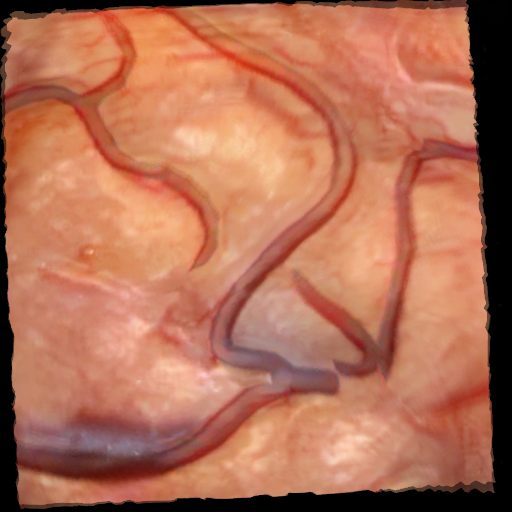
\includegraphics[scale=0.5]{figures/l1/alignment_overlay.png}
  \caption[Registration result with L1 loss]{Overlay of the final registered image on the target image using L1 loss.}
  \label{fig:l1_overlay}
\end{figure}

Figure~\ref{fig:l1_history} shows the corresponding loss history for this optimization run.

\begin{figure}[htpb]
  \centering
  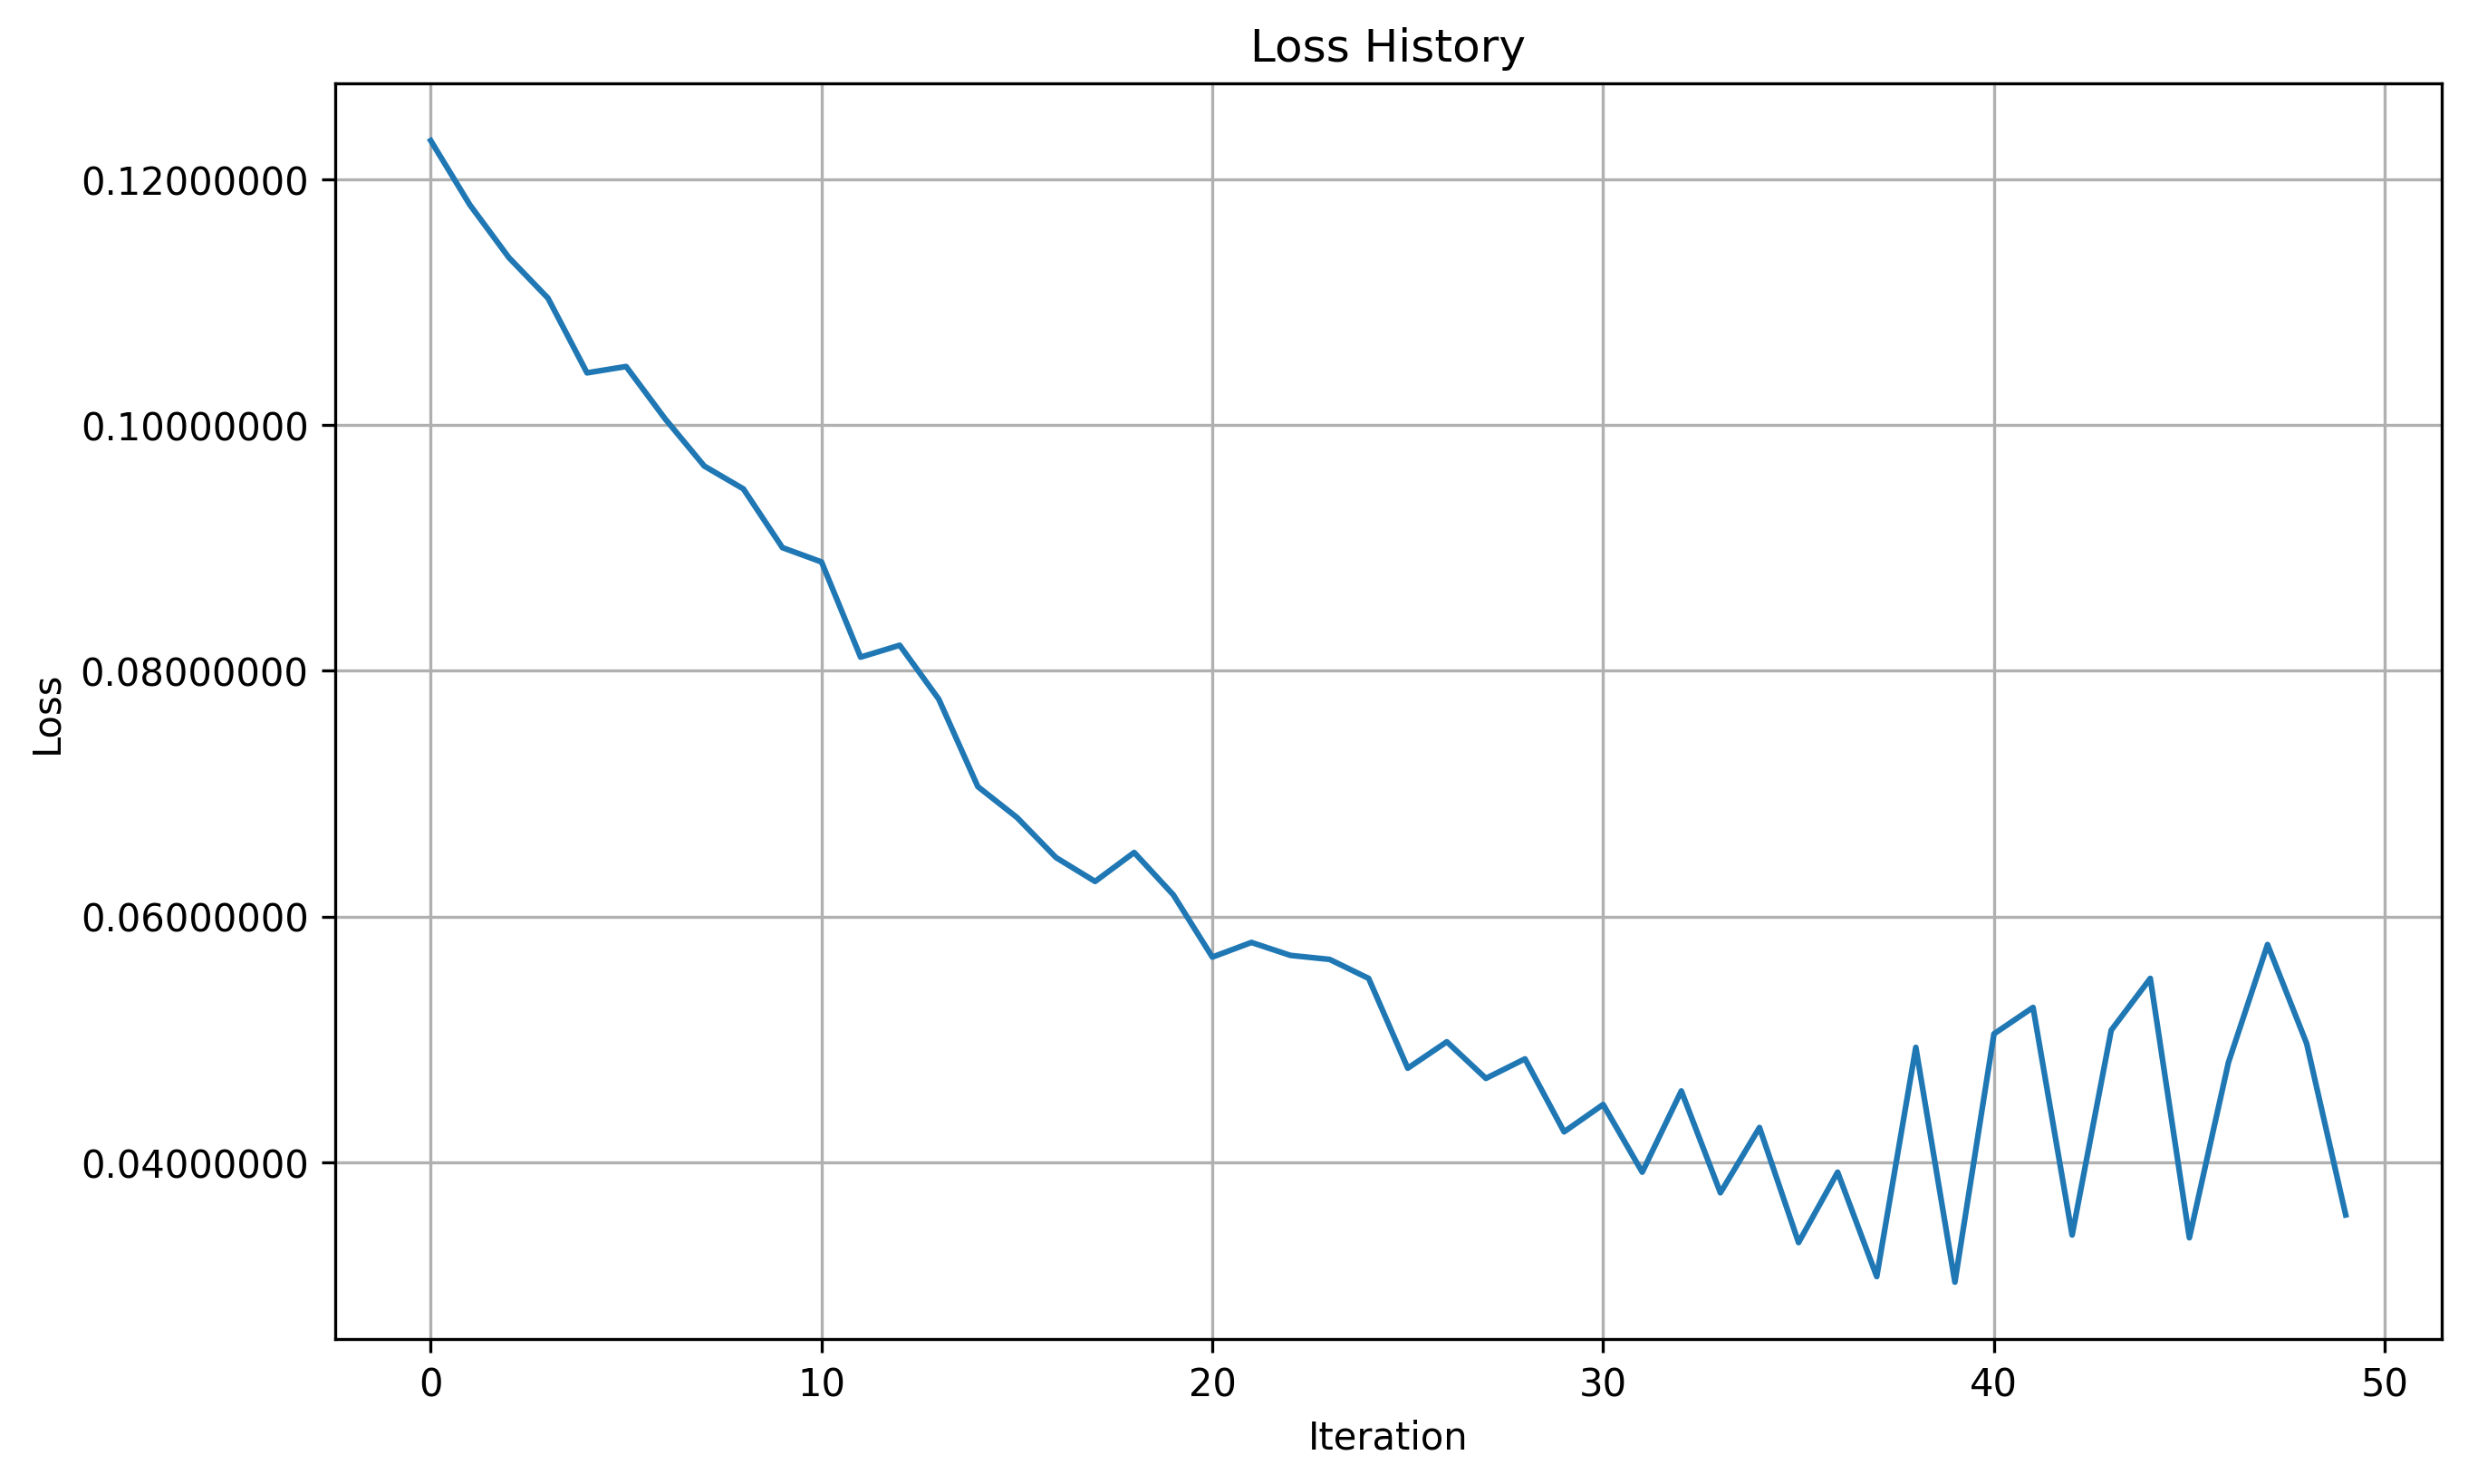
\includegraphics[scale=0.65]{figures/l1/loss_history.png}
  \caption[Loss history for L1 optimization]{Loss history for registration optimization using L1 loss.}
  \label{fig:l1_history}
\end{figure}

The L1 loss function achieved consistent and rapid convergence, reaching its best value at an average of 39 iterations. This suggests that L1 loss may be preferable in scenarios where computational efficiency is a priority.

\section{L2 Loss Performance}

The L2 loss (Mean Squared Error) is the most commonly used loss function in NeRF-based registration approaches, including the original iNeRF implementation. Figure~\ref{fig:l2_overlay} shows an overlay of the final registered image on the target for a representative L2 optimization run.

\begin{figure}[H]
  \centering
  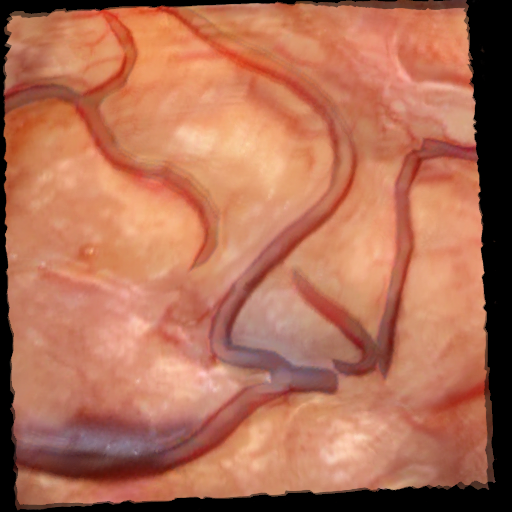
\includegraphics[scale=0.5]{figures/l2/alignment_overlay.png}
  \caption[Registration result with L2 loss]{Overlay of the final registered image on the target image using L2 loss.}
  \label{fig:l2_overlay}
\end{figure}

Figure~\ref{fig:l2_history} shows the corresponding loss history for this optimization run.

\begin{figure}[htpb]
  \centering
  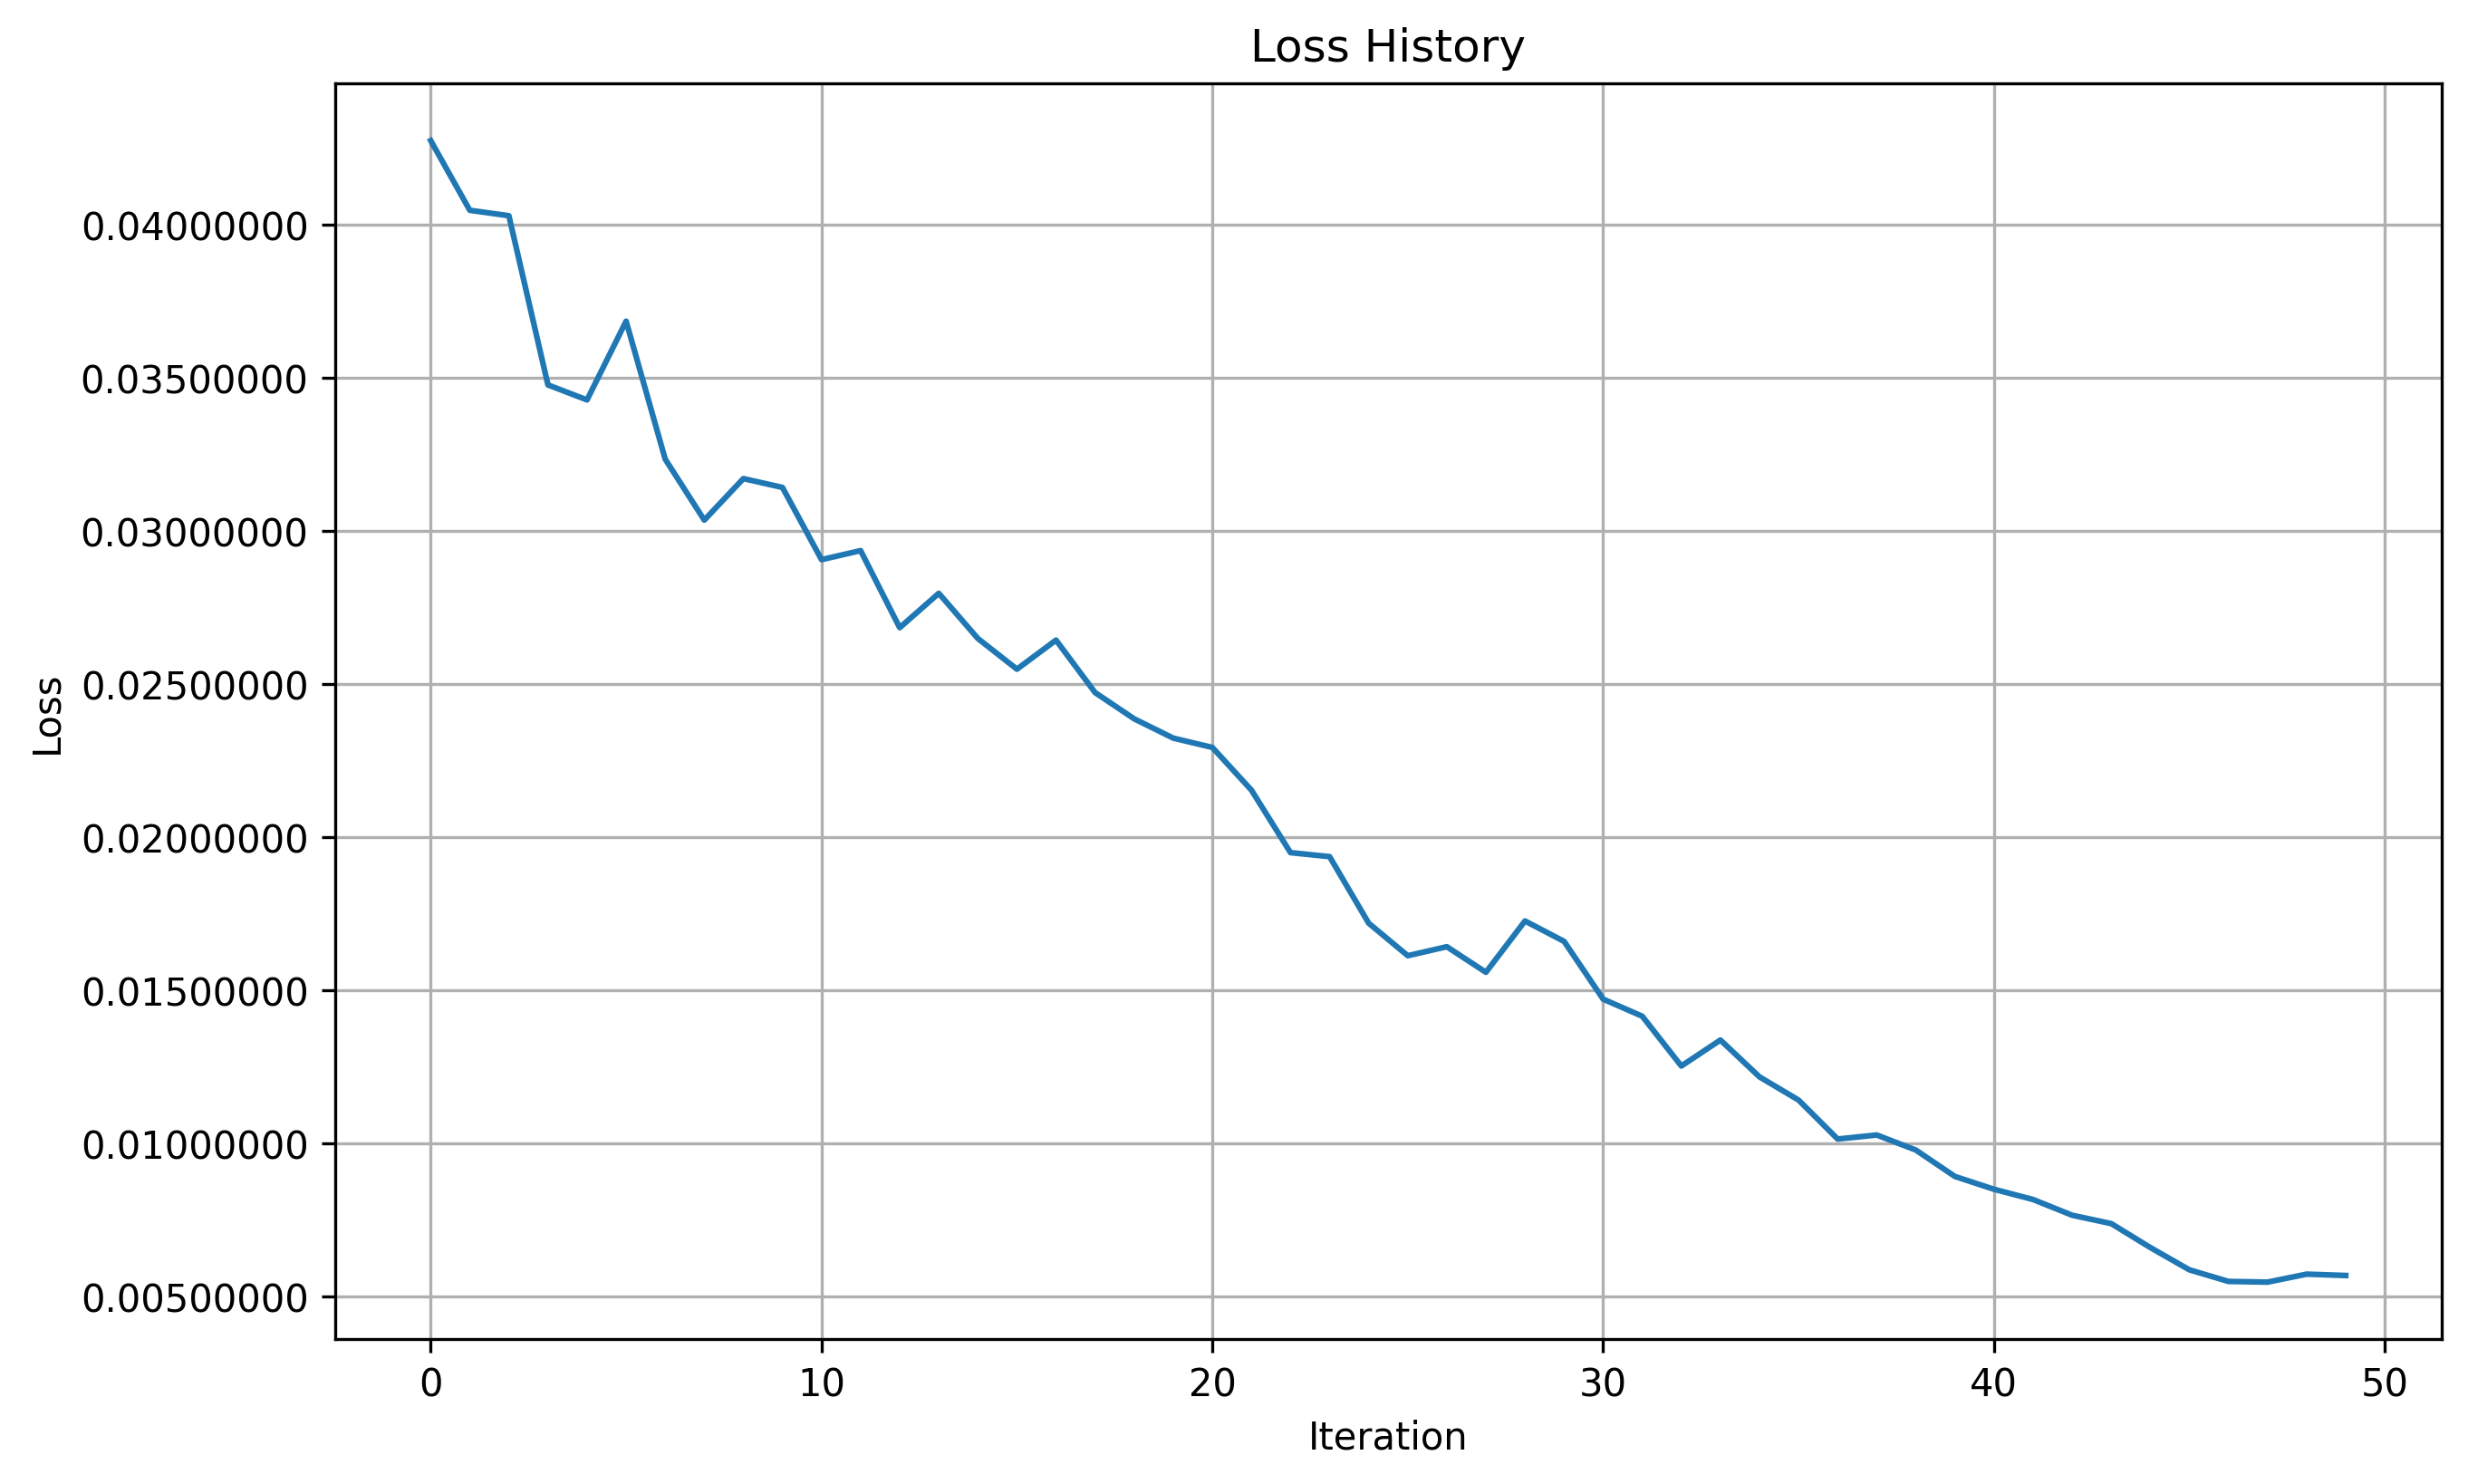
\includegraphics[scale=0.65]{figures/l2/loss_history.png}
  \caption[Loss history for L2 optimization]{Loss history for registration optimization using L2 loss.}
  \label{fig:l2_history}
\end{figure}

The L2 loss required more iterations to converge compared to L1, with an average best loss occurring at iteration 47. This suggests that while L2 can achieve high-quality registration, it may require more computational resources to reach convergence.

\section{Structural Similarity Index Loss Performance}

The Structural Similarity Index (SSIM) loss focuses on preserving structural information rather than pixel-wise differences. Figure~\ref{fig:ssim_overlay} shows an overlay of the final registered image on the target for a representative SSIM optimization run.

\begin{figure}[htpb]
  \centering
  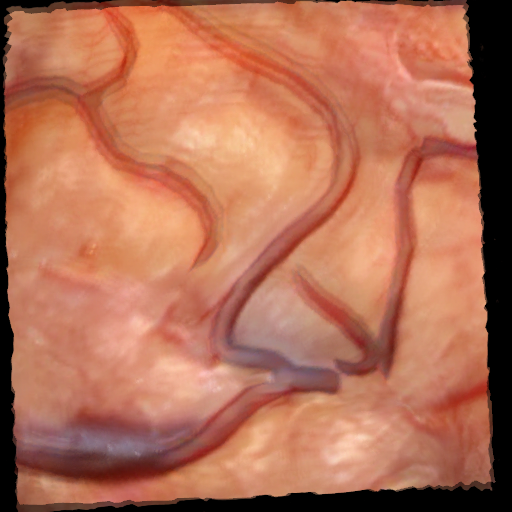
\includegraphics[scale=0.5]{figures/ssim/alignment_overlay.png}
  \caption[Registration result with SSIM loss]{Overlay of the final registered image on the target image using SSIM loss.}
  \label{fig:ssim_overlay}
\end{figure}

Figure~\ref{fig:ssim_history} shows the corresponding loss history for this optimization run.

\begin{figure}[htpb]
  \centering
  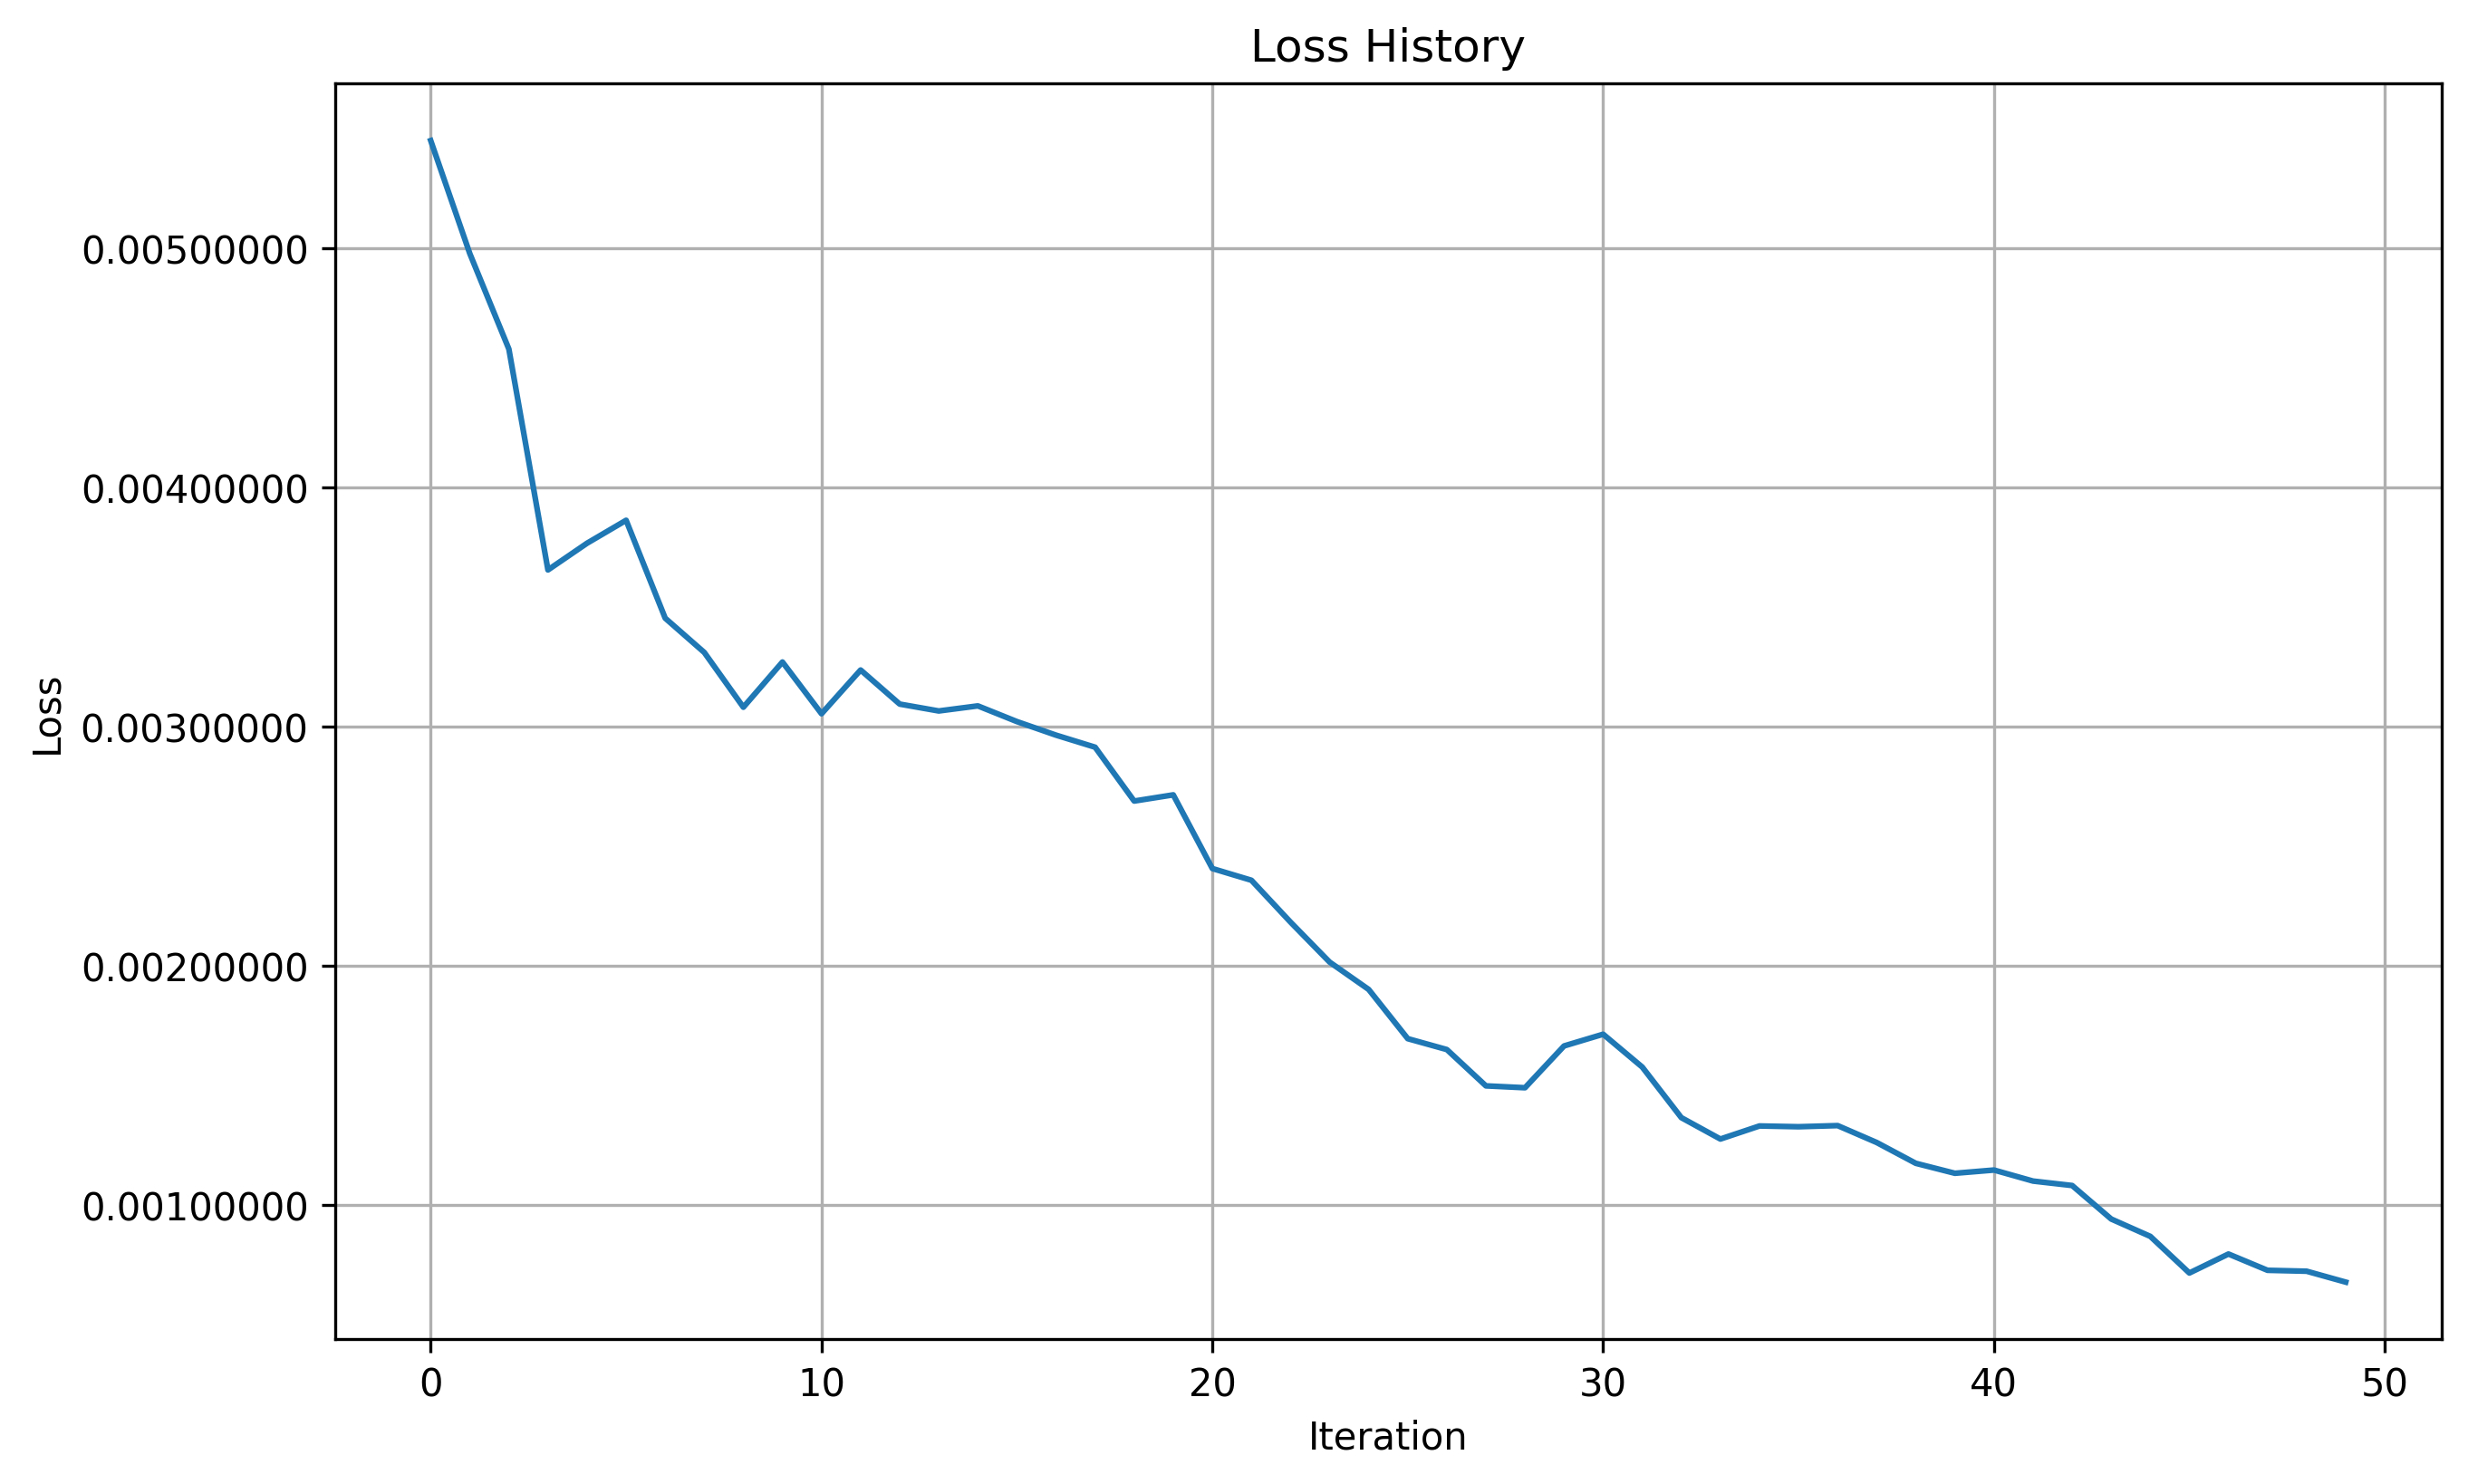
\includegraphics[scale=0.65]{figures/ssim/loss_history.png}
  \caption[Loss history for SSIM optimization]{Loss history for registration optimization using SSIM loss.}
  \label{fig:ssim_history}
\end{figure}

The SSIM loss function required the most iterations to reach its best value, with an average of 49 iterations. This suggests that while SSIM can provide high-quality registration with emphasis on structural correspondence, it may require more computational time to converge fully.

\section{Normalized Cross-Correlation Loss Performance}

Normalized Cross-Correlation (NCC) is often used in multi-modal registration scenarios due to its invariance to linear intensity changes. Figure~\ref{fig:ncc_overlay} shows an overlay of the final registered image on the target for a representative NCC optimization run.

\begin{figure}[htpb]
  \centering
  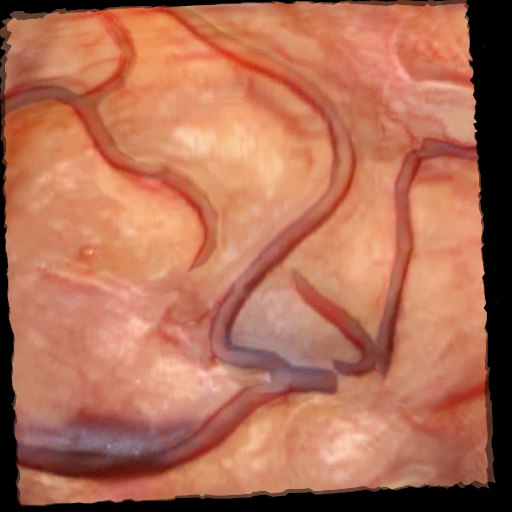
\includegraphics[scale=0.5]{figures/ncc/alignment_overlay.png}
  \caption[Registration result with NCC loss]{Overlay of the final registered image on the target image using NCC loss.}
  \label{fig:ncc_overlay}
\end{figure}

Figure~\ref{fig:ncc_history} shows the corresponding loss history for this optimization run.

\begin{figure}[htpb]
  \centering
  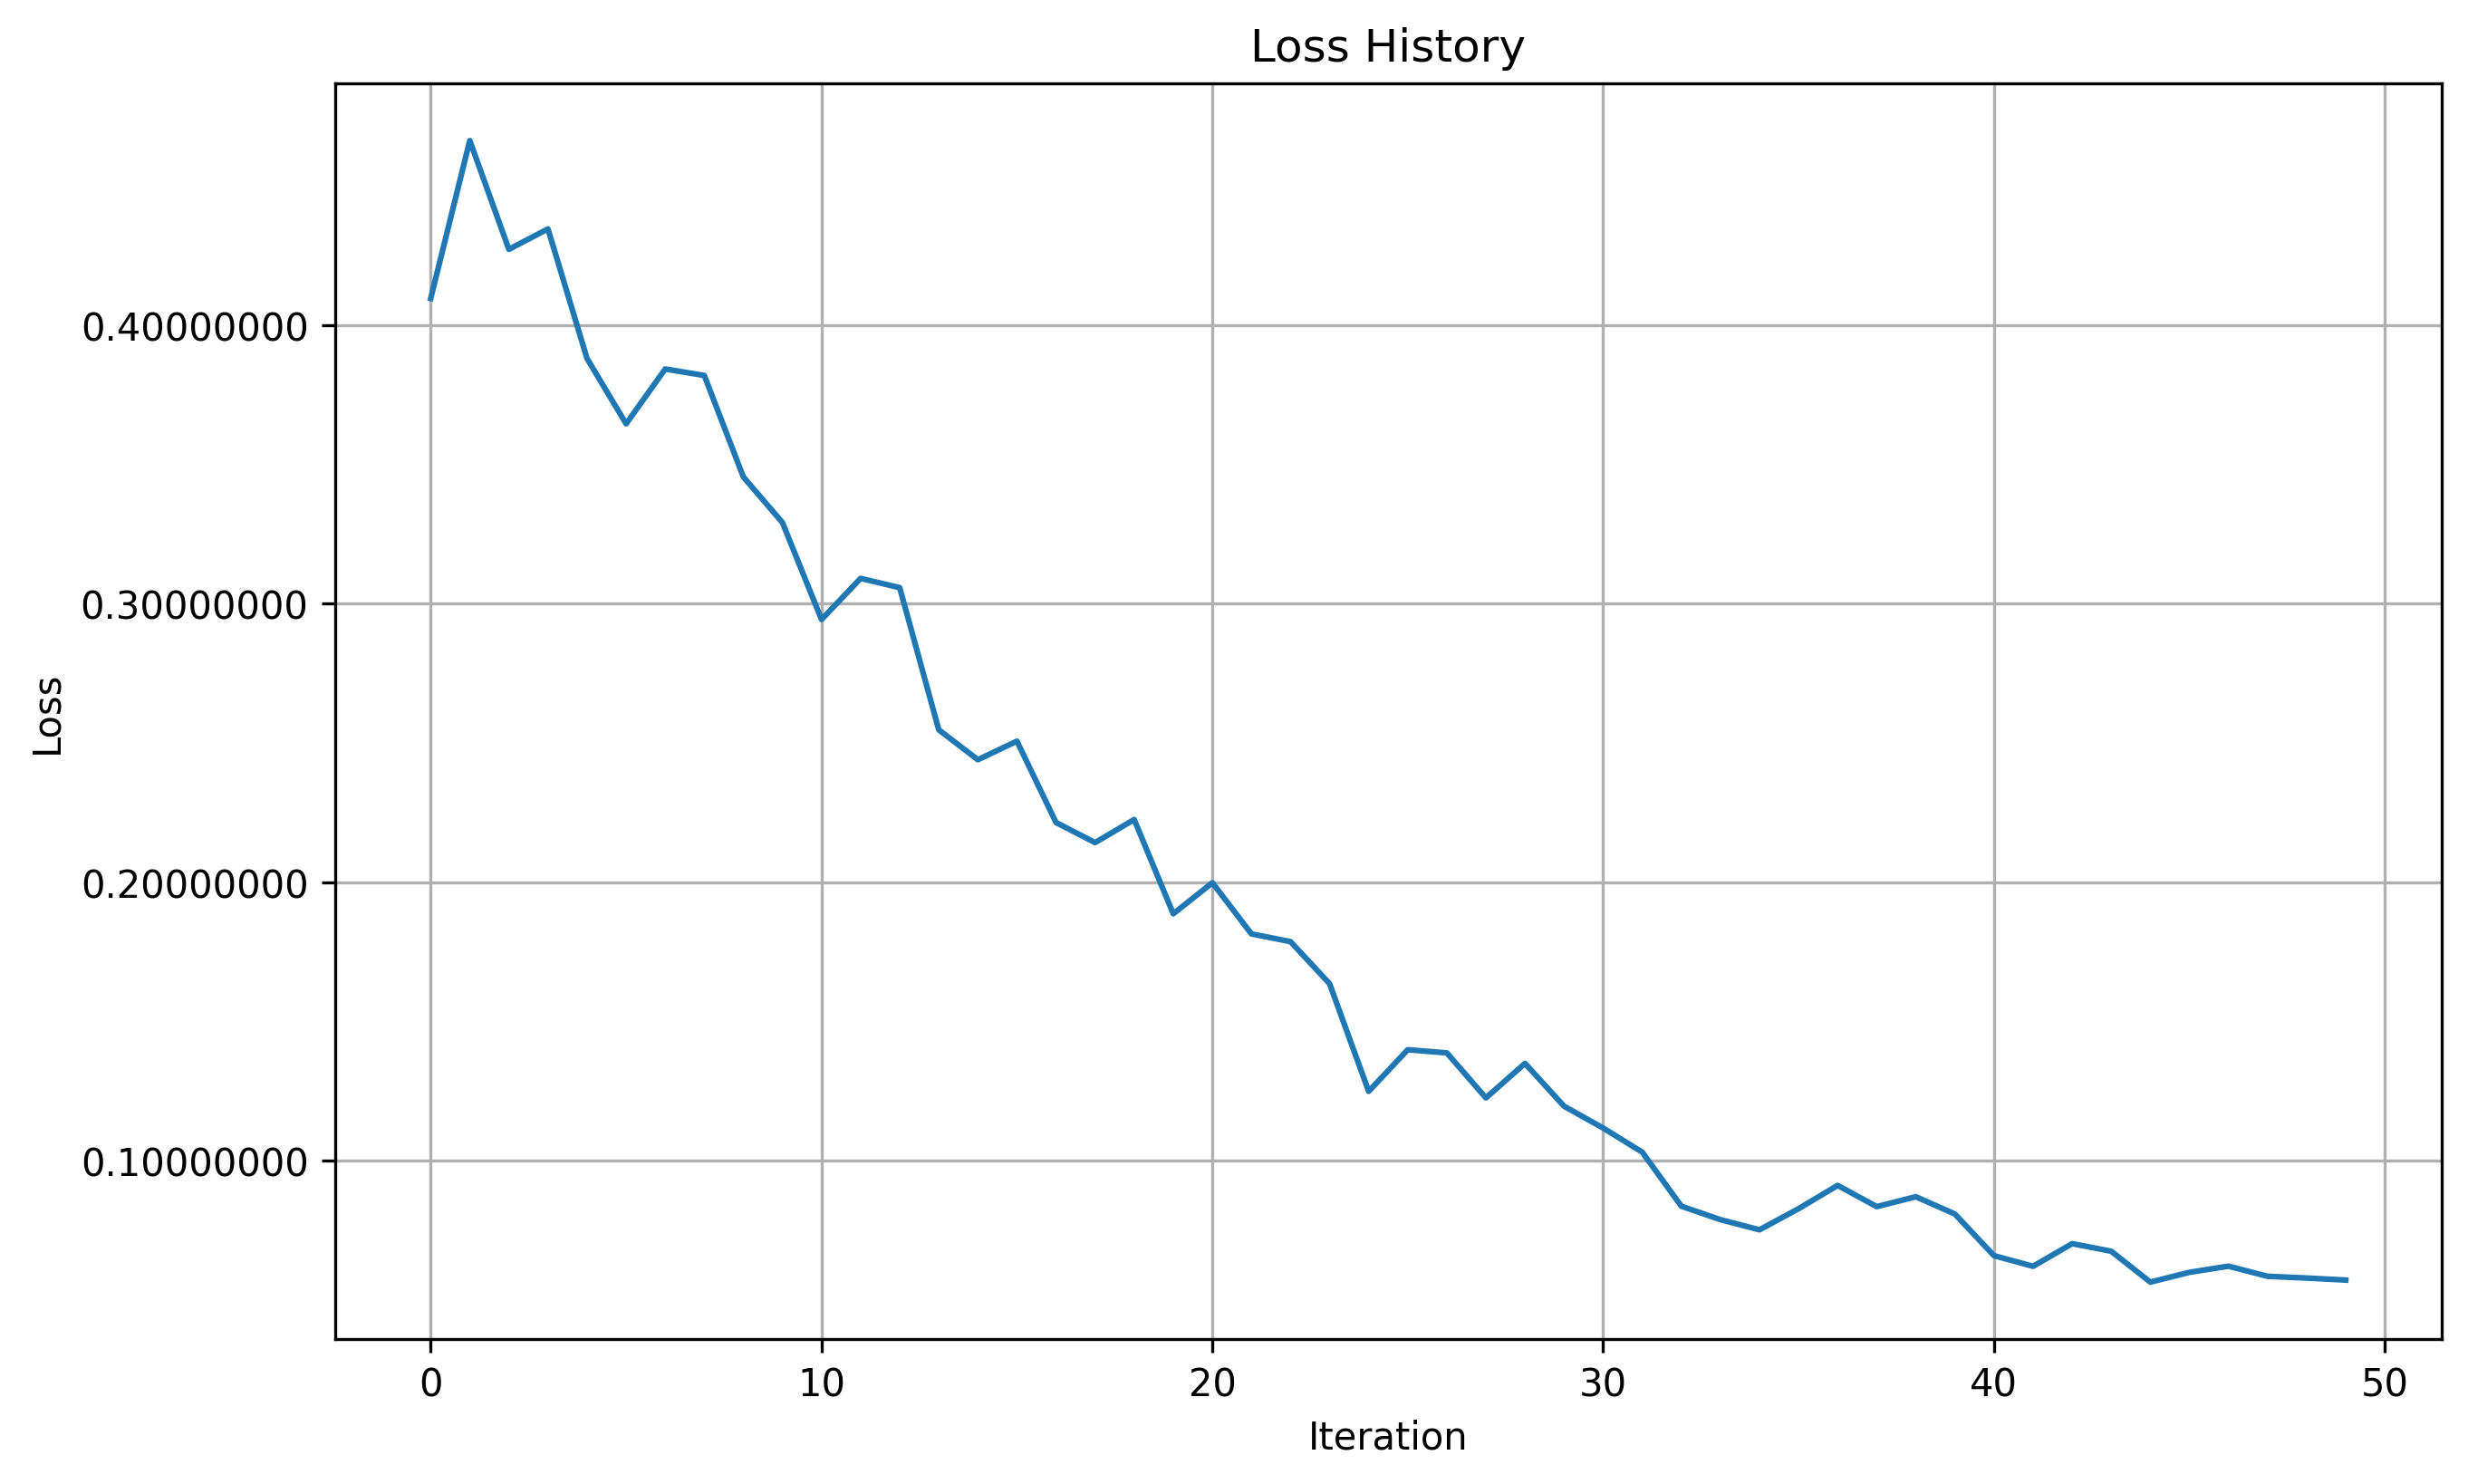
\includegraphics[scale=0.65]{figures/ncc/loss_history.png}
  \caption[Loss history for NCC optimization]{Loss history for registration optimization using NCC loss.}
  \label{fig:ncc_history}
\end{figure}

The NCC loss function demonstrated moderate convergence speed, with its best value occurring at an average of 44 iterations. While slightly slower than L1, NCC showed good stability and robustness to intensity variations.

\section{Mutual Information Loss Performance}

Mutual Information (MI) is a widely used similarity measure for multi-modal registration. Figure~\ref{fig:mi_overlay} shows an overlay of the final registered image on the target for a representative MI optimization run.

\begin{figure}[htpb]
  \centering
  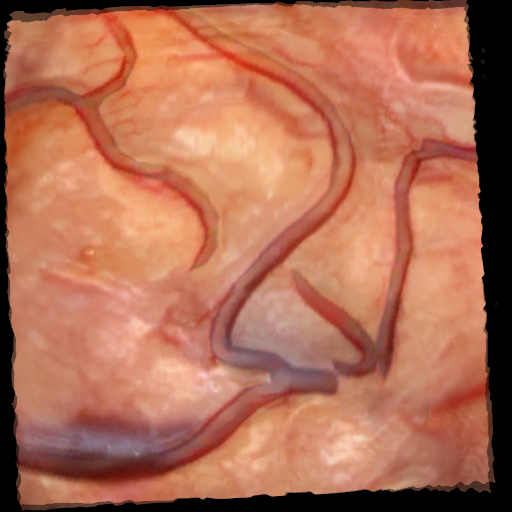
\includegraphics[scale=0.5]{figures/mi/alignment_overlay.png}
  \caption[Registration result with MI loss]{Overlay of the final registered image on the target image using MI loss.}
  \label{fig:mi_overlay}
\end{figure}

Figure~\ref{fig:mi_history} shows the corresponding loss history for this optimization run.

\begin{figure}[htpb]
  \centering
  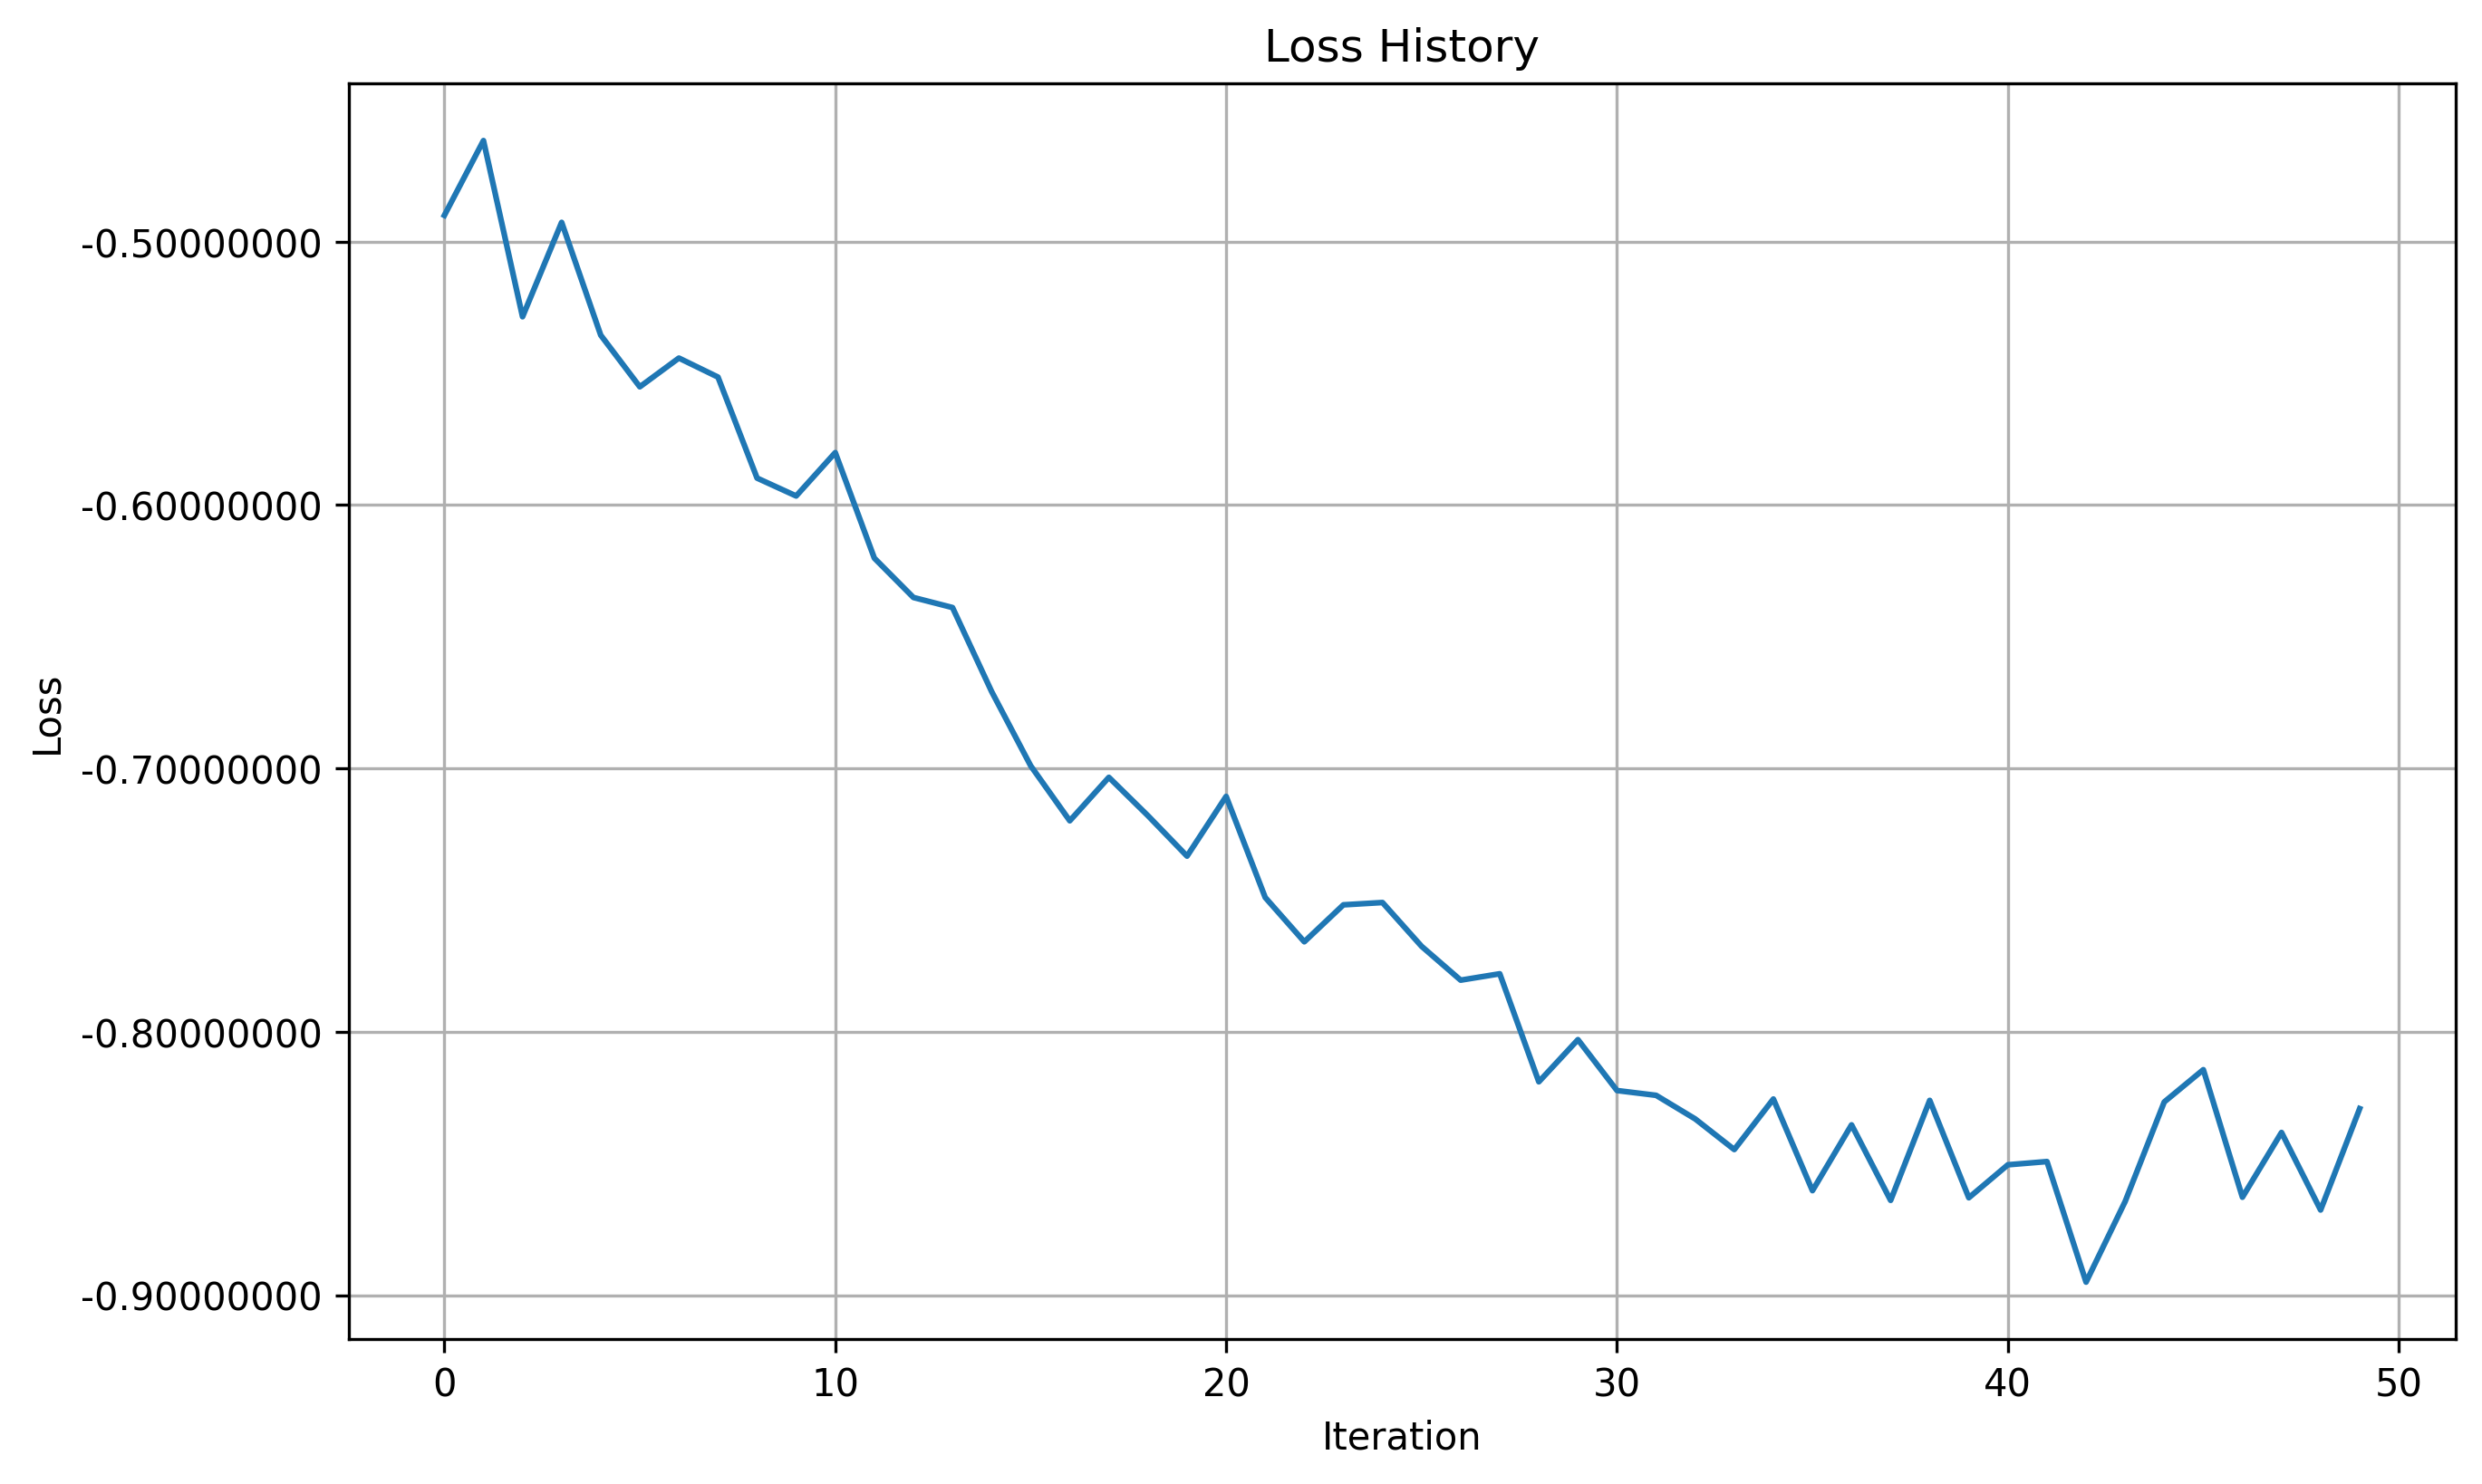
\includegraphics[scale=0.65]{figures/mi/loss_history.png}
  \caption[Loss history for MI optimization]{Loss history for registration optimization using MI loss.}
  \label{fig:mi_history}
\end{figure}

The MI loss function reached its best value at an average of 42 iterations, placing it between L1 and NCC in terms of convergence speed. The more exploratory optimization path of MI may contribute to its robustness in complex registration scenarios.

\section{Limitations and Challenges}

Our implementation and evaluation encountered several limitations and challenges that should be considered:

\begin{itemize}
    \item The use of finite differences for gradient computation, while effective, is computationally more expensive than direct backpropagation.
    
    \item Our experiments assumed perfect NeRF representation of the target object, which is a simplification of real-world scenarios where appearance and lighting variations are significant.
    
    \item The computational cost of registration (averaging around 621-626 seconds for 50 iterations) may be challenging for real-time clinical applications.
    
    \item Our evaluation was limited to a specific set of hyperparameters (learning rate, optimizer, batch size) and may not reflect performance under different conditions.
\end{itemize}

\section{Summary of Findings}

Based on our comprehensive evaluation, we summarize the key findings of our study:

\begin{enumerate}
    \item Our nerfstudio-based implementation provides a flexible framework for experimenting with different loss functions in NeRF-based registration, independent of the specific NeRF architecture.
    
    \item L1 loss demonstrates the fastest convergence among the tested loss functions, making it potentially suitable for time-sensitive applications.
    
    \item Mutual Information and Normalized Cross-Correlation losses exhibit more exploratory behavior during optimization and appear more robust to NeRF rendering artifacts.
    
    \item SSIM loss shows slower convergence but maintains focus on structural correspondence, which may be beneficial for preserving anatomical structures.
    
    \item All five loss functions eventually achieve visually satisfactory registration, suggesting that the choice of loss function may depend on specific application requirements such as speed, robustness, or structural preservation.
\end{enumerate}

These results highlight the importance of loss function selection in NeRF-based registration and provide a foundation for future work in this area. 
% !TeX root = ../main.tex

\chapter{Discussion}\label{chap:discussion}

In this chapter, we interpret the results of our experiments, discuss the caveats associated with our experimental setup, highlight the limitations of our current approach, and suggest directions for future research.

\section{Interpretation of Results}

\subsection{Loss Function Performance}
Our experiments revealed distinct performance characteristics associated with each evaluated loss function. L1 loss consistently demonstrated faster convergence compared to other loss functions, notably achieving quicker reductions in error. Additionally, both L1 and L2 losses exhibited smoother and more direct convergence trajectories, which may indicate their suitability for tasks requiring rapid and stable alignment, such as intraoperative scenarios.

In contrast, Structural Similarity Index (SSIM), Normalized Cross-Correlation (NCC), and Mutual Information (MI) demonstrated more explorative behavior during initial iterations, characterized by fluctuating, "jiggly" optimization paths. This behavior suggests these losses may explore the parameter space more thoroughly at the cost of slower initial convergence. Mutual Information and NCC, in particular, showed more oscillations, reflecting their sensitivity to variations in pixel intensities but also their potential robustness to certain types of noise or distortions.

\section{Caveats of the Experimental Setup}\label{sec:caveats}

The experimental design involved several key simplifications that limit direct translation to clinical practice:

\begin{itemize}
    \item \textbf{Perfect NeRF assumption:} Both target and iterative images were synthesized from the same pre-trained NeRF, eliminating realistic factors such as lighting variations, surgical environment noise, and intraoperative tissue deformation. Therefore, while the current setup provides a controlled environment to evaluate the registration method, it overestimates real-world accuracy.
    
    \item \textbf{Finite Differences for Gradient Calculation:} Due to complexity in directly implementing backpropagation through InstantNGP-based NeRF models, finite differences were utilized as a workaround. While effective in proof-of-concept scenarios, this method is computationally expensive and less precise than automatic differentiation.
    
    \item \textbf{Constant Camera Distance and Fixed Initialization:} The experimental scenario assumed a fixed camera distance and a manually chosen initial position that always provided a partial view of the target region. This is unrealistic in surgical settings, where initial camera positioning can vary significantly, and occlusions may frequently occur.
\end{itemize}

\section{Limitations}\label{sec:limitations}

Several limitations affect the current approach:

\begin{itemize}
    \item \textbf{Computational Efficiency:} Finite differences-based gradient estimation significantly increases computational load, limiting real-time clinical applicability.

    \item \textbf{Assumption of Model Accuracy:} The assumption that NeRF perfectly captures brain geometry and appearance neglects inevitable inaccuracies in the preoperative model and intraoperative tissue deformation and appearance changes.

    \item \textbf{Initialization Sensitivity:} The current method heavily depends on the initial camera pose selection, affecting convergence speed and reliability.

    \item \textbf{Generalization to Clinical Data:} Experiments conducted entirely with synthetic images derived from a single NeRF model may not generalize well to real clinical images due to differences in lighting, texture, and anatomical variability.
\end{itemize}

\section{Future Work}\label{sec:futurework}

Future directions for improving and extending the proposed neural registration approach include:

\begin{itemize}
    \item \textbf{Automatic Differentiation Integration:} Replacing finite differences with automatic differentiation methods to significantly improve computational efficiency and stability.

    \item \textbf{Gaussian Splats:} Investigating Gaussian Splats as an alternative representation, offering faster rendering, fewer visual artifacts, and potentially superior registration performance.

    \item \textbf{Enhanced NeRF Models:} Incorporating hypernetwork-based methods to better match the NeRF model's density and appearance to actual intraoperative conditions, addressing the oversimplification in the current setup.

    \item \textbf{Robust Initialization Strategies:} Developing methods for automatic or semi-automatic selection of robust initial camera poses, thus reducing sensitivity to starting conditions and improving reliability.

    \item \textbf{Hybrid Loss Functions:} Exploring combined or adaptive loss functions to leverage the strengths of multiple similarity metrics, potentially achieving superior registration accuracy and robustness.

    \item \textbf{Clinical Validation:} Extending evaluation to realistic clinical or phantom datasets to assess practical applicability, robustness against real-world variability, and identification of clinical relevance.
\end{itemize}

Addressing these areas in future research will pave the way for practical clinical applications of NeRF-based intraoperative registration, enhancing surgical precision and patient outcomes.

% !TeX root = ../main.tex

\chapter{Conclusion}\label{chapter:conclusion}

This study introduced an enhanced intraoperative registration method using Neural Radiance Fields (NeRFs), highlighting the critical role of differentiable implicit representations in accurately aligning preoperative and intraoperative brain surface images. By developing a flexible, NeRF-model agnostic implementation inspired by iNeRF, the algorithm facilitates robust and customizable intraoperative registration workflows.

We conducted an extensive exploration of various loss functions (L1, L2, Structural Similarity Index, Normalized Cross-Correlation, and Mutual Information) and analyzed their impacts on the convergence behavior and registration accuracy. The results demonstrated that L1 and L2 losses provide rapid and stable convergence, making them suitable for clinical scenarios requiring efficiency and reliability. On the other hand, Mutual Information and Normalized Cross-Correlation, despite their less direct convergence trajectories, offer greater flexibility in scenarios where robustness to imaging variations might be advantageous.

Despite these promising findings, the study acknowledges critical simplifications and assumptions. The current simulation assumes an idealized scenario where the NeRF perfectly represents the intraoperative brain surface, eliminating realistic noise, lighting variations, and inaccuracies. Additionally, the computational performance remains limited by the finite difference gradient estimation method implemented as a workaround for gradient propagation challenges in InstantNGP models.

Future work should focus on overcoming these limitations by:
\begin{itemize}
\item Developing more realistic NeRF models that capture intraoperative variability in brain appearance through enhanced coloring techniques, potentially leveraging hypernetworks for more robust representations.
\item Transitioning from finite difference-based gradient calculations to efficient direct backpropagation methods to improve optimization speed and efficiency.
\end{itemize}

Further exploration into faster and visually superior methods, such as Gaussian Splatting, represents a promising direction for significantly improving registration performance and computational efficiency, ultimately advancing the accuracy and reliability of intraoperative brain registration in clinical settings.



\appendix{}

\chapter{Implementation Details}\label{appendix:implementation}

This appendix provides additional technical details about the implementation of the NeRF-based registration approach described in this thesis. The code is available at: \url{https://github.com/maxfehrentz/style-ngp}.

\section{Software Implementation}

The neural registration framework described in this thesis was implemented in Python using PyTorch. This section provides a detailed description of the key components of the implementation.

\subsection{Image Processing and Conversion}

The following utility functions handle image processing and conversion between different formats:

\begin{lstlisting}[language=Python]
def image_to_tensor(image_path, device) -> torch.Tensor:
    # Open the image using PIL
    image = Image.open(image_path).convert("RGB")
    
    # Define the transform to convert the image to a PyTorch tensor
    transform = transforms.ToTensor()  # This will convert to a tensor with shape (C, H, W)
    
    # Apply the transform
    tensor = transform(image)  # Shape will be (3, 512, 512)
    
    # Permute the tensor to get shape (512, 512, 3)
    tensor = tensor.permute(1, 2, 0).to(device)
    
    return tensor.detach().requires_grad_(False)

def show_image(tensor):
    plt.figure(figsize=(5, 5))
    plt.imshow(tensor.detach().cpu().numpy())
    plt.axis('off')
    plt.show()
\end{lstlisting}

\subsection{iNeRF Optimization}

The core of the registration framework is the \texttt{iNeRFOptimizerBatchedFD} class, which implements inverse NeRF optimization with batched finite differences for gradient computation. This approach allows for the estimation of camera pose parameters by minimizing the difference between a rendered NeRF view and a target image.

\subsubsection{Initialization}

The optimizer is initialized with the following parameters:

\begin{lstlisting}[language=Python]
def __init__(
    self,
    experiment_name, 
    nerf_model, 
    target_image,
    initial_pose,
    dataparser_matrix,
    dataparser_scale,
    camera_params,
    loss_fn = nn.MSELoss(),
    lr=0.001,
    num_iterations=1000,
    config_path=None
):
\end{lstlisting}

Parameters include:
\begin{itemize}
    \item \texttt{experiment\_name}: Name for tracking and saving results
    \item \texttt{nerf\_model}: The pre-trained NeRF model
    \item \texttt{target\_image}: The target image to register against
    \item \texttt{initial\_pose}: Initial camera pose estimate
    \item \texttt{dataparser\_matrix} and \texttt{dataparser\_scale}: Transform parameters for coordinate system alignment
    \item \texttt{camera\_params}: Camera intrinsic parameters
    \item \texttt{loss\_fn}: Loss function for comparing rendered and target images
    \item \texttt{lr}: Learning rate
    \item \texttt{num\_iterations}: Maximum number of optimization iterations
\end{itemize}

\subsubsection{Optimization Process}

The optimization uses finite differences to compute gradients rather than automatic differentiation. This is implemented in the \texttt{optimize\_step} method:

\begin{lstlisting}[language=Python]
def optimize_step(self, batch_size=4, debug=True):
    # Zero gradients
    self.optimizer.zero_grad()
    
    # Get current pose parameters
    pose = self.pose_param.detach().clone()
    
    # Compute loss for current pose
    original_loss, pred_rgb = self.compute_loss_no_grad(pose)
    
    # Small epsilon for finite differences
    eps = 1e-4
    
    # Compute gradients using finite differences in batches
    grad = torch.zeros_like(pose)
    
    # Flatten the pose for easier batch processing
    num_params = pose.numel()
    
    # Use coordinate indexing to track which element we're perturbing
    coords = [(i, j) for i in range(pose.shape[0]) for j in range(pose.shape[1])]
    
    # Process in batches
    for batch_idx in range(0, num_params, batch_size):
        batch_coords = coords[batch_idx:min(batch_idx+batch_size, num_params)]
        
        # Create a batch of perturbed poses
        batch_poses = []
        for i, j in batch_coords:
            perturbed_pose = pose.clone()
            perturbed_pose[i, j] += eps
            batch_poses.append(perturbed_pose)
        
        # Stack poses into a batch
        batch_poses_tensor = torch.stack(batch_poses)
        
        # Compute losses for all poses in the batch
        batch_losses = self.compute_batch_losses(batch_poses_tensor)
        
        # Calculate gradients
        for idx, (i, j) in enumerate(batch_coords):
            grad[i, j] = (batch_losses[idx] - original_loss) / eps
    
    # Manually set gradients
    self.pose_param.grad = grad
    
    # Perform optimization step
    self.optimizer.step()
    
    return original_loss.item(), pred_rgb
\end{lstlisting}

This batched approach to finite differences significantly improves performance by computing multiple perturbed poses in parallel.

\subsubsection{Camera Creation and Loss Computation}

The optimizer creates cameras from pose matrices and computes losses between rendered and target images:

\begin{lstlisting}[language=Python]
def create_camera_from_pose(self, pose):
    camera = Cameras(
        camera_to_worlds=pose.unsqueeze(0),
        fx=self.camera_params["fl_x"],
        fy=self.camera_params["fl_y"],
        cx=self.camera_params["cx"],
        cy=self.camera_params["cy"],
        camera_type=CameraType.PERSPECTIVE,
        height=self.camera_params["h"],
        width=self.camera_params["w"],
    )
    return camera

def compute_loss_no_grad(self, pose):
    with torch.no_grad():
        # Create camera with the given pose
        camera = self.create_camera_from_pose(pose)
        
        # Get outputs using the model's built-in method for rendering
        outputs = self.nerf_model.get_outputs_for_camera(camera)
        
        # Compute loss
        pred_rgb, image = self.nerf_model.renderer_rgb.blend_background_for_loss_computation(
            pred_image=outputs["rgb"],
            pred_accumulation=outputs["accumulation"],
            gt_image=self.target_image,
        )
        
        loss = self.nerf_model.rgb_loss(image, pred_rgb)
        
    return loss, pred_rgb
\end{lstlisting}

\subsection{Loss Functions}

Multiple loss functions were implemented and compared for registration accuracy:

\subsubsection{Standard Losses}
\begin{lstlisting}[language=Python]
# L1 and L2 losses
l1_loss = nn.L1Loss()
l2_loss = nn.MSELoss()
huber_loss = nn.SmoothL1Loss(beta=0.5)
\end{lstlisting}

\subsubsection{Structural Similarity Index Loss}
\begin{lstlisting}[language=Python]
class StructuralSimilarityIndexLoss(nn.Module):
    def __init__(self):
        super(StructuralSimilarityIndexLoss, self).__init__()
    
    def forward(self, x, y):
        # Rearrange dimensions if needed
        if x.dim() == 3:  # [H, W, C]
            # Rearrange to [1, C, H, W]
            x = x.permute(2, 0, 1).unsqueeze(0)
            y = y.permute(2, 0, 1).unsqueeze(0)
        
        return 1 - pytorch_msssim.ssim(x, y)
\end{lstlisting}

\subsubsection{Normalized Cross-Correlation Loss}
\begin{lstlisting}[language=Python]
class NormalizedCrossCorrelationLoss(nn.Module):
    def __init__(self):
        super(NormalizedCrossCorrelationLoss, self).__init__()
        
    def forward(self, x, y):
        # Ensure proper dimensions
        if x.dim() == 3:  # [H, W, C]
            # Handle each channel separately and average
            channels = x.shape[2]
            ncc_sum = 0.0
            
            for c in range(channels):
                x_c = x[..., c].flatten()
                y_c = y[..., c].flatten()
                ncc_sum += self._compute_ncc(x_c, y_c)
                
            ncc = ncc_sum / channels
        else:  # Assume [B, C, H, W]
            batch_size, channels = x.shape[0], x.shape[1]
            ncc_sum = 0.0
            
            for b in range(batch_size):
                channel_ncc = 0.0
                for c in range(channels):
                    x_bc = x[b, c].flatten()
                    y_bc = y[b, c].flatten()
                    channel_ncc += self._compute_ncc(x_bc, y_bc)
                ncc_sum += channel_ncc / channels
                
            ncc = ncc_sum / batch_size
        
        # Convert to loss (1 - NCC since NCC=1 is perfect correlation)
        return 1.0 - ncc
    
    def _compute_ncc(self, x, y):
        # Mean centering
        x_centered = x - x.mean()
        y_centered = y - y.mean()
        
        # Compute normalization factors
        x_norm = torch.sqrt(torch.sum(x_centered ** 2) + 1e-8)
        y_norm = torch.sqrt(torch.sum(y_centered ** 2) + 1e-8)
        
        # Compute NCC
        ncc = torch.sum(x_centered * y_centered) / (x_norm * y_norm)
        
        # Ensure result is in [-1, 1] range
        return torch.clamp(ncc, -1.0, 1.0)
\end{lstlisting}

\subsubsection{Mutual Information Loss}
\begin{lstlisting}[language=Python]
class MutualInformationLoss(nn.Module):
    def __init__(self, bins=32, sigma=0.1):
        super(MutualInformationLoss, self).__init__()
        self.bins = bins
        self.sigma = sigma
        self.epsilon = 1e-10  # Small constant to avoid log(0)
        
    def forward(self, x, y):
        # Ensure proper dimensions
        if x.dim() == 3:  # [H, W, C]
            x_flat = x.reshape(-1)
            y_flat = y.reshape(-1)
        else:  # Assume [B, C, H, W]
            x_flat = x.reshape(x.size(0), -1)
            y_flat = y.reshape(y.size(0), -1)
            
        # Scale to [0, 1] if not already
        if x_flat.max() > 1.0 or x_flat.min() < 0.0:
            x_flat = (x_flat - x_flat.min()) / (x_flat.max() - x_flat.min() + self.epsilon)
        if y_flat.max() > 1.0 or y_flat.min() < 0.0:
            y_flat = (y_flat - y_flat.min()) / (y_flat.max() - y_flat.min() + self.epsilon)
            
        # Compute mutual information
        mi_score = self._compute_mutual_information(x_flat, y_flat)
        
        # Return negative MI as we want to minimize loss
        return -mi_score
\end{lstlisting}

\subsection{Experiment Tracking and Visualization}

The implementation includes comprehensive experiment tracking and visualization features:

\begin{itemize}
    \item Automatic creation of experiment directories
    \item Saving of intermediate and final renders
    \item Tracking of loss history and optimization progress
    \item Generation of visualization overlays for alignment quality assessment
    \item JSON-based tracking of all experiment parameters and results
\end{itemize}

\subsection{Experimental Evaluation}

The implementation supports systematic evaluation of different loss functions and registration parameters. Example experiments include:

\begin{lstlisting}[language=Python]
# Experiment 1: L1 loss
inerf_optimizer = iNeRFOptimizerBatchedFD(
    experiment_name="0_065_cat5_2_l1",
    nerf_model=nerf_model,
    target_image=target_image,
    initial_pose=final_initial_pose,
    dataparser_matrix=dataparser_matrix,
    dataparser_scale=dataparser_scale,
    camera_params=camera_params,
    loss_fn=l1_loss,
    lr=0.01,
    num_iterations=50,
    config_path=config_path
)

# Experiment 2: L2 loss
inerf_optimizer = iNeRFOptimizerBatchedFD(
    experiment_name="0_065_cat5_2_l2",
    ...
    loss_fn=l2_loss,
    ...
)

# Experiment 3: SSIM loss
inerf_optimizer = iNeRFOptimizerBatchedFD(
    experiment_name="0_065_cat5_2_ssim",
    ...
    loss_fn=structural_similarity_index_loss,
    ...
)

# Additional experiments with NCC and MI loss functions
\end{lstlisting}

\section{Hyperparameter Settings}\label{appendix:hyperparameters}

This section details the key hyperparameters used in our neural registration framework and their effects on the registration process.

\subsection{Optimization Hyperparameters}

\begin{itemize}
    \item \textbf{Learning Rate}: We primarily used learning rates between 0.001 and 0.01. Higher learning rates can lead to faster convergence but may cause instability, while lower rates provide more stable but slower optimization. For most experiments, a learning rate of 0.01 provided good results.
    
    \item \textbf{Number of Iterations}: Experiments were conducted with 50-1000 iterations. For evaluation purposes, 50 iterations were often sufficient to demonstrate the effectiveness of different loss functions, while longer runs (500-1000 iterations) were used for final results to ensure convergence.
    
    \item \textbf{Batch Size}: The finite difference gradient computation used batch sizes between 4 and 12. Larger batch sizes increased memory usage but significantly improved computation time by parallelizing the evaluation of perturbed poses.
    
    \item \textbf{Epsilon Value}: A value of $1e^{-4}$ was used for finite difference calculations. This represents the small perturbation applied to each parameter when computing gradients numerically.
\end{itemize}

\subsection{Loss Function Hyperparameters}

Different loss functions require specific hyperparameters:

\begin{itemize}
    \item \textbf{Mutual Information Loss}:
    \begin{itemize}
        \item Bins: 32 (controls the discretization of intensity values)
        \item Sigma: 0.1 (kernel width for soft binning)
    \end{itemize}
    
    \item \textbf{Structural Similarity Loss}:
    \begin{itemize}
        \item Uses default parameters from the PyTorch SSIM implementation
    \end{itemize}
    
    \item \textbf{Huber Loss}:
    \begin{itemize}
        \item Beta: 0.5 (controls the transition point between L1 and L2 behavior)
    \end{itemize}
\end{itemize}

\subsection{Camera Model Parameters}

Camera intrinsic parameters used in the experiments:

\begin{itemize}
    \item \textbf{Image Resolution}: 512×512 pixels
    \item \textbf{Focal Length}: fl\_x = fl\_y = 955.4050067376327
    \item \textbf{Principal Point}: cx = cy = 256.0
    \item \textbf{Field of View}: 0.5235987755982988 radians (approximately 30 degrees)
    \item \textbf{Distortion Parameters}: All set to 0 (no distortion modeling)
\end{itemize}

\subsection{Performance Considerations}

The choice of hyperparameters significantly impacts both registration accuracy and computational efficiency:

\begin{itemize}
    \item Increasing batch size from 4 to 12 resulted in approximately 3× speedup in gradient computation with minimal impact on convergence.
    
    \item The choice of loss function often had a greater impact on registration accuracy than tuning other optimization parameters. For most medical image registration scenarios, Normalized Cross-Correlation (NCC) and Structural Similarity Index (SSIM) provided better results than L1 or L2 losses due to their robustness to intensity variations.
    
    \item Optimization progress was tracked at intervals of 10-50 iterations to enable early stopping if needed, though most experiments ran to completion.
    
    \item Rendering resolution remained fixed at 512×512 for all experiments, as this provided a good balance between detail and computational efficiency.
\end{itemize}

\subsection{Experimental Configurations}

For systematic comparison of different registration approaches, we consistently used the following configuration across experiments:

\begin{itemize}
    \item Initial pose perturbation magnitudes were consistent across all compared methods
    \item All methods used the same NeRF model trained with identical hyperparameters
    \item 5 repeated trials with different random initializations were conducted for each experimental configuration to account for optimization variability
    \item Target images were selected from held-out test views not used during NeRF training
\end{itemize}

The hyperparameter values listed above represent our final configuration after extensive experimentation. These settings provided a good balance between registration accuracy, convergence reliability, and computational efficiency across the datasets used in this study.

\chapter{Glossary}\label{appendix:glossary}

\begin{description}
    \item[Brain Shift] The deformation of brain tissue during surgery due to factors such as cerebrospinal fluid drainage, gravity, and surgical manipulations, which reduces the accuracy of rigid registration methods.
    
    \item[Cross-Modal Registration] The process of aligning images from different imaging modalities, such as preoperative MRI data with intraoperative camera images, which presents unique challenges due to differences in information content, geometric representation, and visual appearance.
    
    \item[Finite Difference] A numerical method for computing gradients by evaluating a function at multiple perturbed points, used in this thesis to overcome limitations with gradient flow in the computational graph.
    
    \item[Hypernetwork] A neural network that generates parameters for another neural network, used to adapt the appearance of NeRF renderings while preserving geometric structure.
    
    \item[iNeRF (Inverse Neural Radiance Field)] A method that inverts Neural Radiance Fields for pose estimation by optimizing camera parameters through backpropagation to minimize the difference between rendered and target images.
    
    \item[Intraoperative] Occurring during a surgical procedure, specifically referring to the registration and imaging processes that take place while surgery is being performed.
    
    \item[L1 Loss] A loss function that calculates the absolute difference between pixels in two images, often more robust to outliers than L2 loss.
    
    \item[L2 Loss] Also known as Mean Squared Error (MSE), a loss function that calculates the squared Euclidean distance between two images, commonly used in image registration due to its simplicity and differentiability.
    
    \item[Model Agnosticism] The quality of an implementation that works with multiple model variants without being tied to a specific architecture, allowing for greater flexibility and comparative evaluation.
    
    \item[Mutual Information (MI)] An information-theoretic measure that quantifies the mutual dependence between two random variables by evaluating their joint and marginal probability distributions, particularly useful for cross-modal registration where the relationship between image intensities is complex.
    
    \item[NeRF (Neural Radiance Field)] An implicit neural representation that maps 3D coordinates and viewing directions to color and volume density, enabling novel view synthesis of complex scenes through a continuous, differentiable function optimized using volume rendering techniques.
    
    \item[Nerfstudio] An implementation-agnostic framework for developing and deploying Neural Radiance Field models, which combines advances from various NeRF variants for improved performance.
    
    \item[Normalized Cross-Correlation (NCC)] A similarity measure that calculates the correlation between two signals normalized by their standard deviations, making it robust to linear intensity transformations between images.
    
    \item[Registration] The process of aligning two or more datasets into a common coordinate system, essential in neurosurgery for ensuring accurate spatial correspondence between preoperative imaging data and the patient's anatomy.
    
    \item[Structural Similarity Index (SSIM)] A perceptual metric that quantifies image similarity based on changes in structural information, luminance, and contrast, modeled after the human visual system.
    
    \item[Style Transfer] The process of applying the visual style of one image to the content of another image, used in cross-modal registration to bridge appearance gaps between different imaging modalities.
\end{description}

\microtypesetup{protrusion=false}
\listoffigures{}
\listoftables{}
\microtypesetup{protrusion=true}
\printglossaries
\printbibliography

\end{document}
